

\textbf{Study design}

    \centering
    \includegraphics[width=0.75\linewidth]{src/pictures/StudyData/Study_design.drawio.drawio-1.drawio.png}

\textbf{Words that are tested}


    \centering
    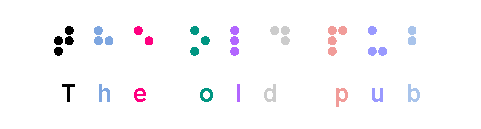
\includegraphics[width=.75\linewidth]{src/pictures/braille_prestudy_characters.drawio.pdf}


 
\textbf{RQ1: Is there a significant difference in the learning rate between affective and discriminative touch.}

\textbf{(General Participant Data)}

\resizebox{\columnwidth}{!}{
    \begin{tabular}{|c|c|c|c|} \hline 
        Gender & Age & Dominant Hand & Previous Braille Knowledge\\ \hline 
        M & 27 & R & No\\ \hline 
        M & 27 & R & No\\ \hline 
        M & 22 & R & No\\ \hline 
        M & 22 & R & No\\ \hline 
        M & 26 & R & No\\ \hline 
        M & 27 & R & No\\ \hline 
        M & 28 & R & No\\ \hline 
        W & 28 & R & No\\ \hline 
        W & 27 & R & No\\ \hline 
        M & 30 & L & No\\ \hline 
        M & 25 & R & No\\ \hline 
        W & 55 & R & No\\ \hline
    \end{tabular}}


(Check the concentration of the participants, if the data is valid)

    \centering
    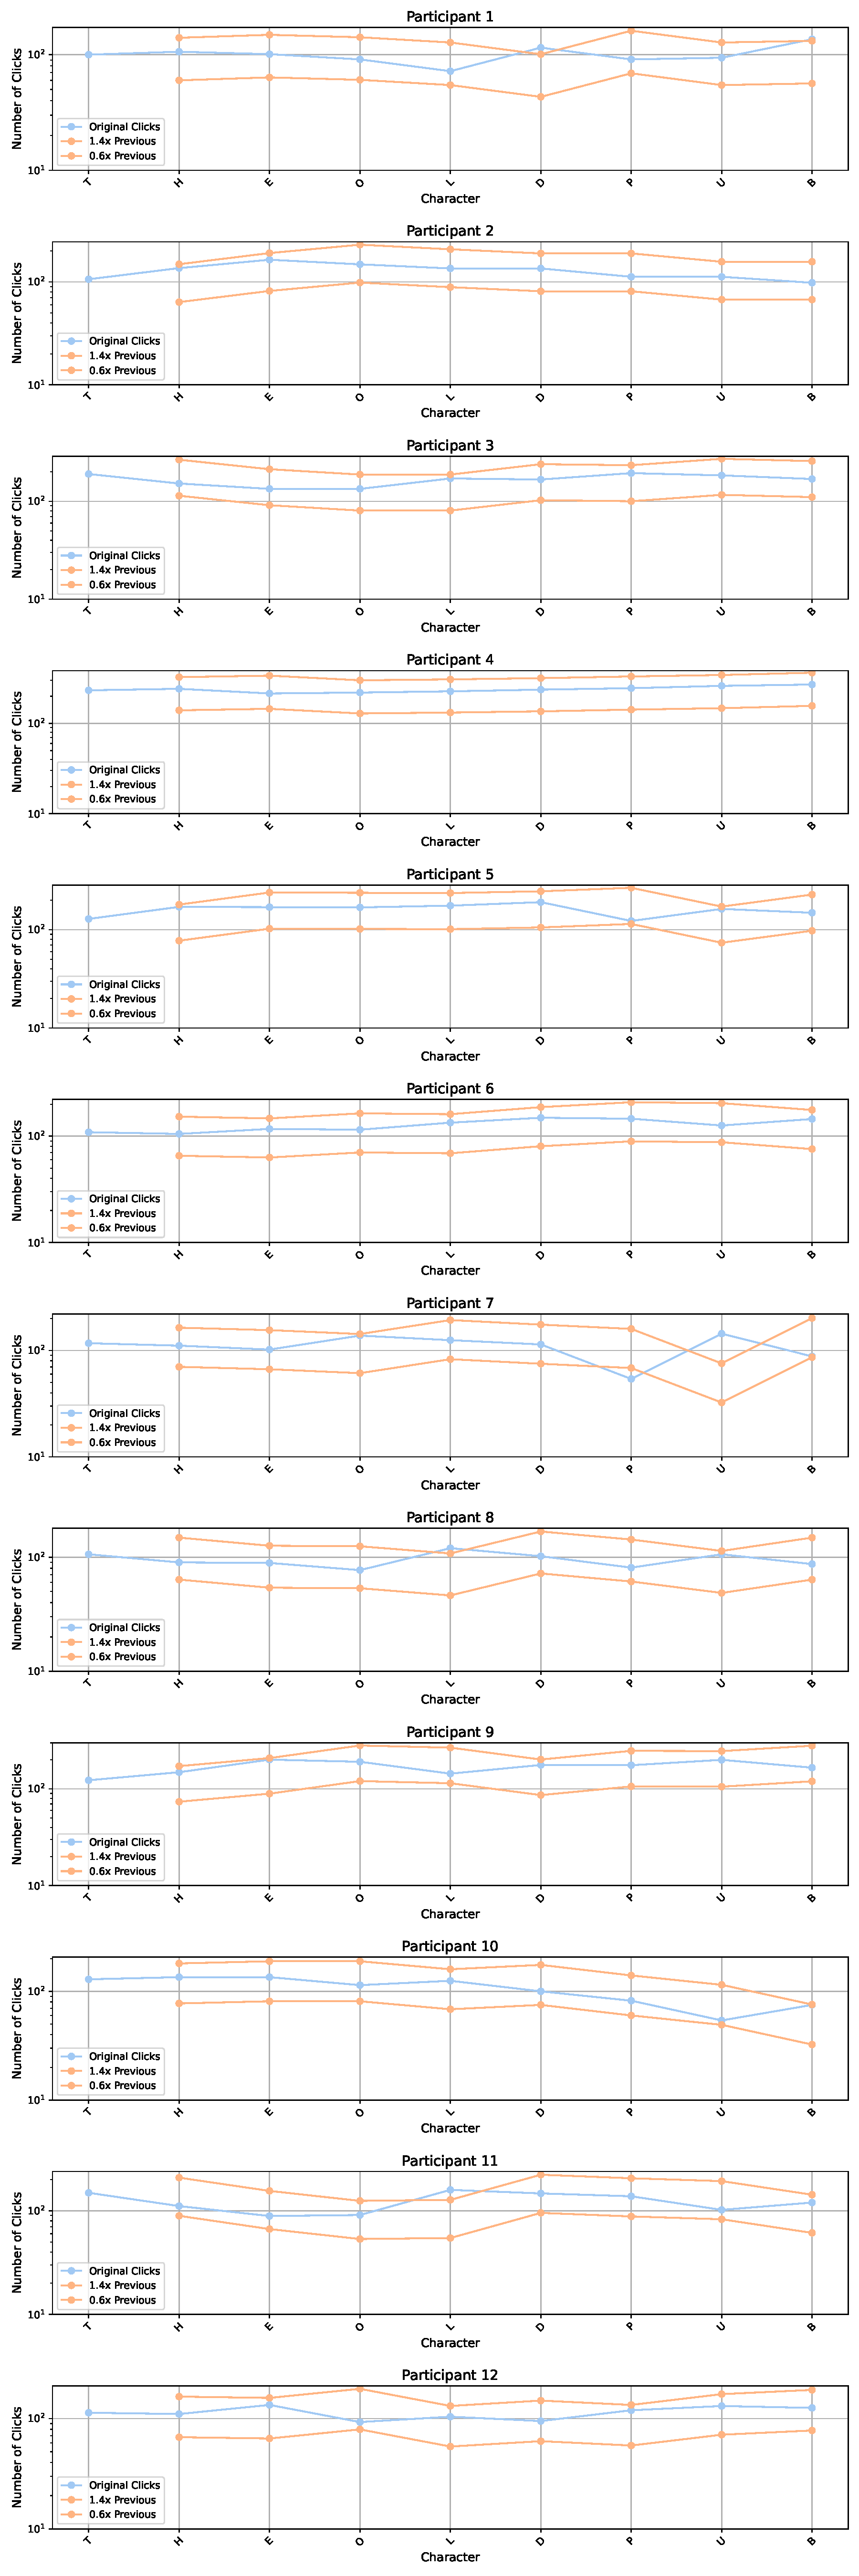
\includegraphics[width=0.5\linewidth]{src/pictures/Study1Data/participantPlots_study1.pdf}



\begin{enumerate}
    \item Learning one Braille word consisting out of three Braille characters with one affective/discriminative touch Stimuli passively (\braille{t} (T),\braille{h} (H),\braille{e} (E),\braille{o} (O),\braille{l} (L),\braille{d} (D), \braille{p} (P), \braille{u} (U),\braille{b} (B)) with a test after each character.
    
        \centering
        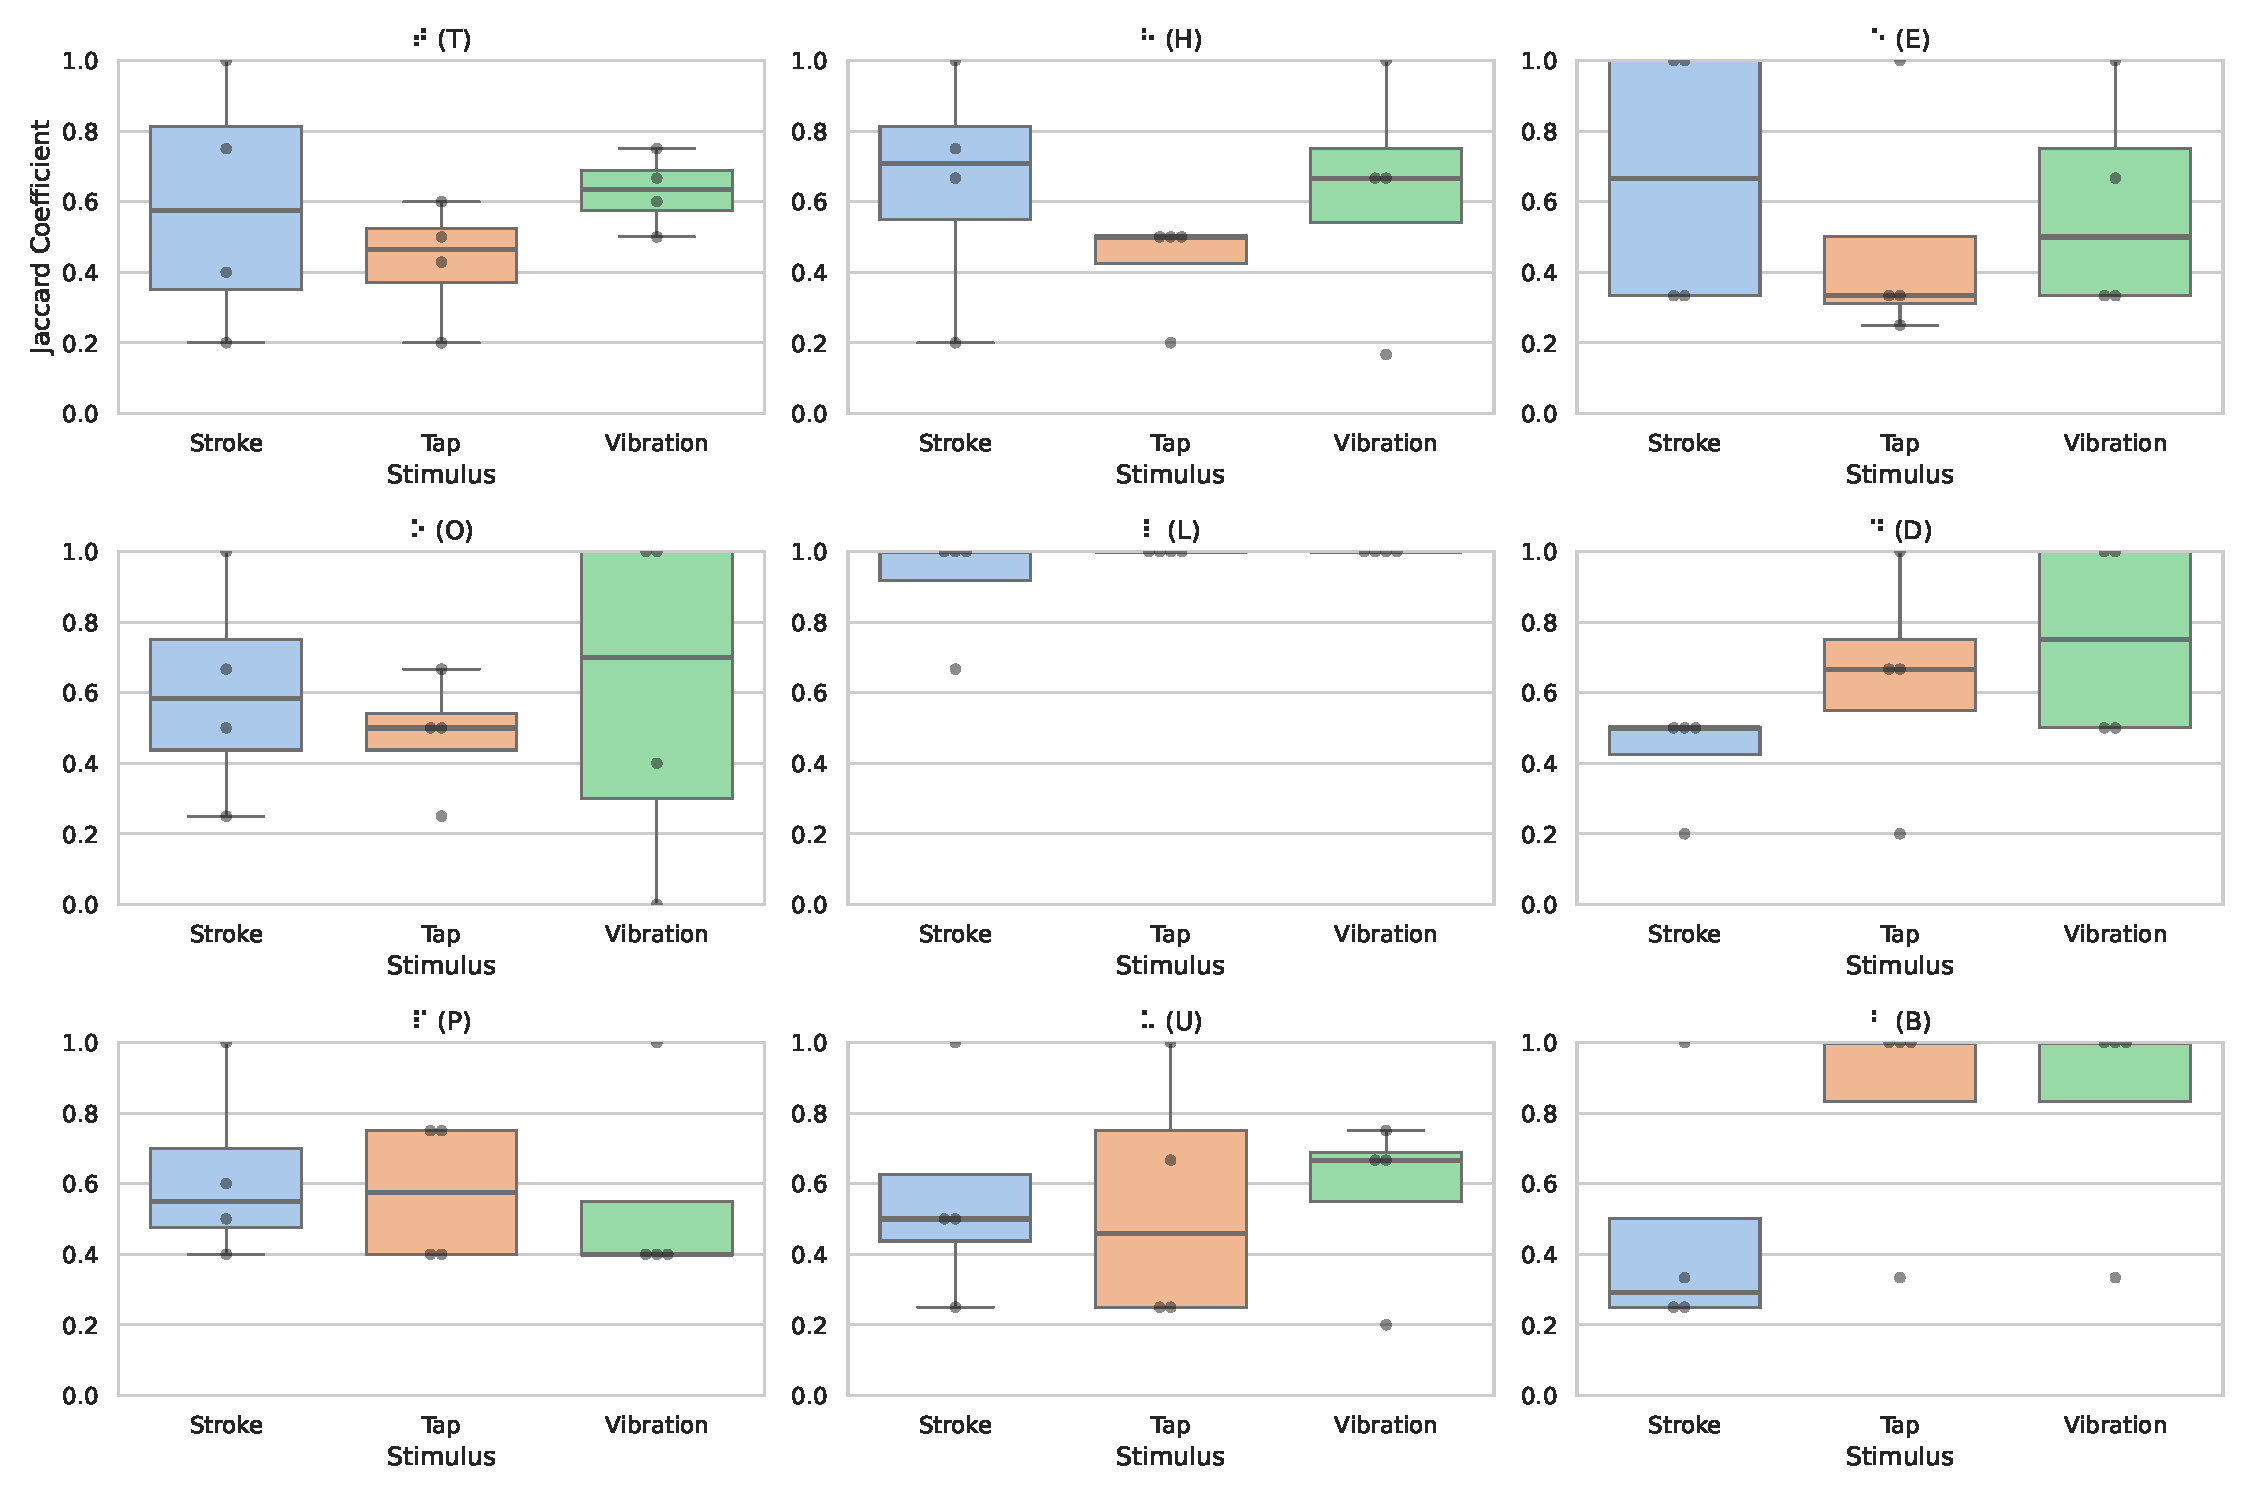
\includegraphics[width=\linewidth]{src/pictures/Study1Data/study1_learning_results.pdf}

\begin{table}[ht]
\resizebox{\columnwidth}{!}{
\centering
\begin{tabular}{|l|l|l|l|l|}
\hline
\textbf{Question} & \textbf{Test Statistic} & \textbf{p-value}  &\textbf{Significance}           &\textbf{Effect Size}\\ \hline
\braille{t}(\textbf{T})& 1.9406 & 0.3790  &Not Significant &0.1764\\ \hline
\braille{h}(\textbf{H})& 2.2817& 0.3195&Not Significant &0.2074\\ \hline
\braille{e}(\textbf{E})& 1.1068 & 0.5750  &Not Significant &0.1006\\ \hline
\braille{o}(\textbf{O})& 0.2790& 0.8698&Not Significant &0.0254\\ \hline
\braille{l}(\textbf{L})& 2.0000 & 0.3679  &Not Significant &0.1818\\ \hline
\braille{d}(\textbf{D})& 2.9298& 0.2311&Not Significant &0.2663\\ \hline
\braille{p}(\textbf{P})& 0.7068 & 0.7023  &Not Significant &0.0643\\ \hline
\braille{u}(\textbf{U})& 0.0299& 0.9852&Not Significant &0.0027\\ \hline
\braille{b}(\textbf{B})& 3.6667 & 0.1599  &Not Significant &0.3333\\ \hline
\end{tabular}}
\caption{Results of Kruskal-Wallis significance tests for the different Braille characters during learning with a $\eta^2$ Effect Size.}
\label{table:learning_significance_results_firstStudy_nonParam}
\end{table}
B = stroking bad
, D = stroking bad
h,e = stroking good
h = tab bad,E auch
P = vibration bad

    \item After one word was learned with a Stimuli, we conducted a word-tests the Braille word (\braille{THE} (THE), \braille{old} (OLD), \braille{pub} (PUB)).

        \centering
        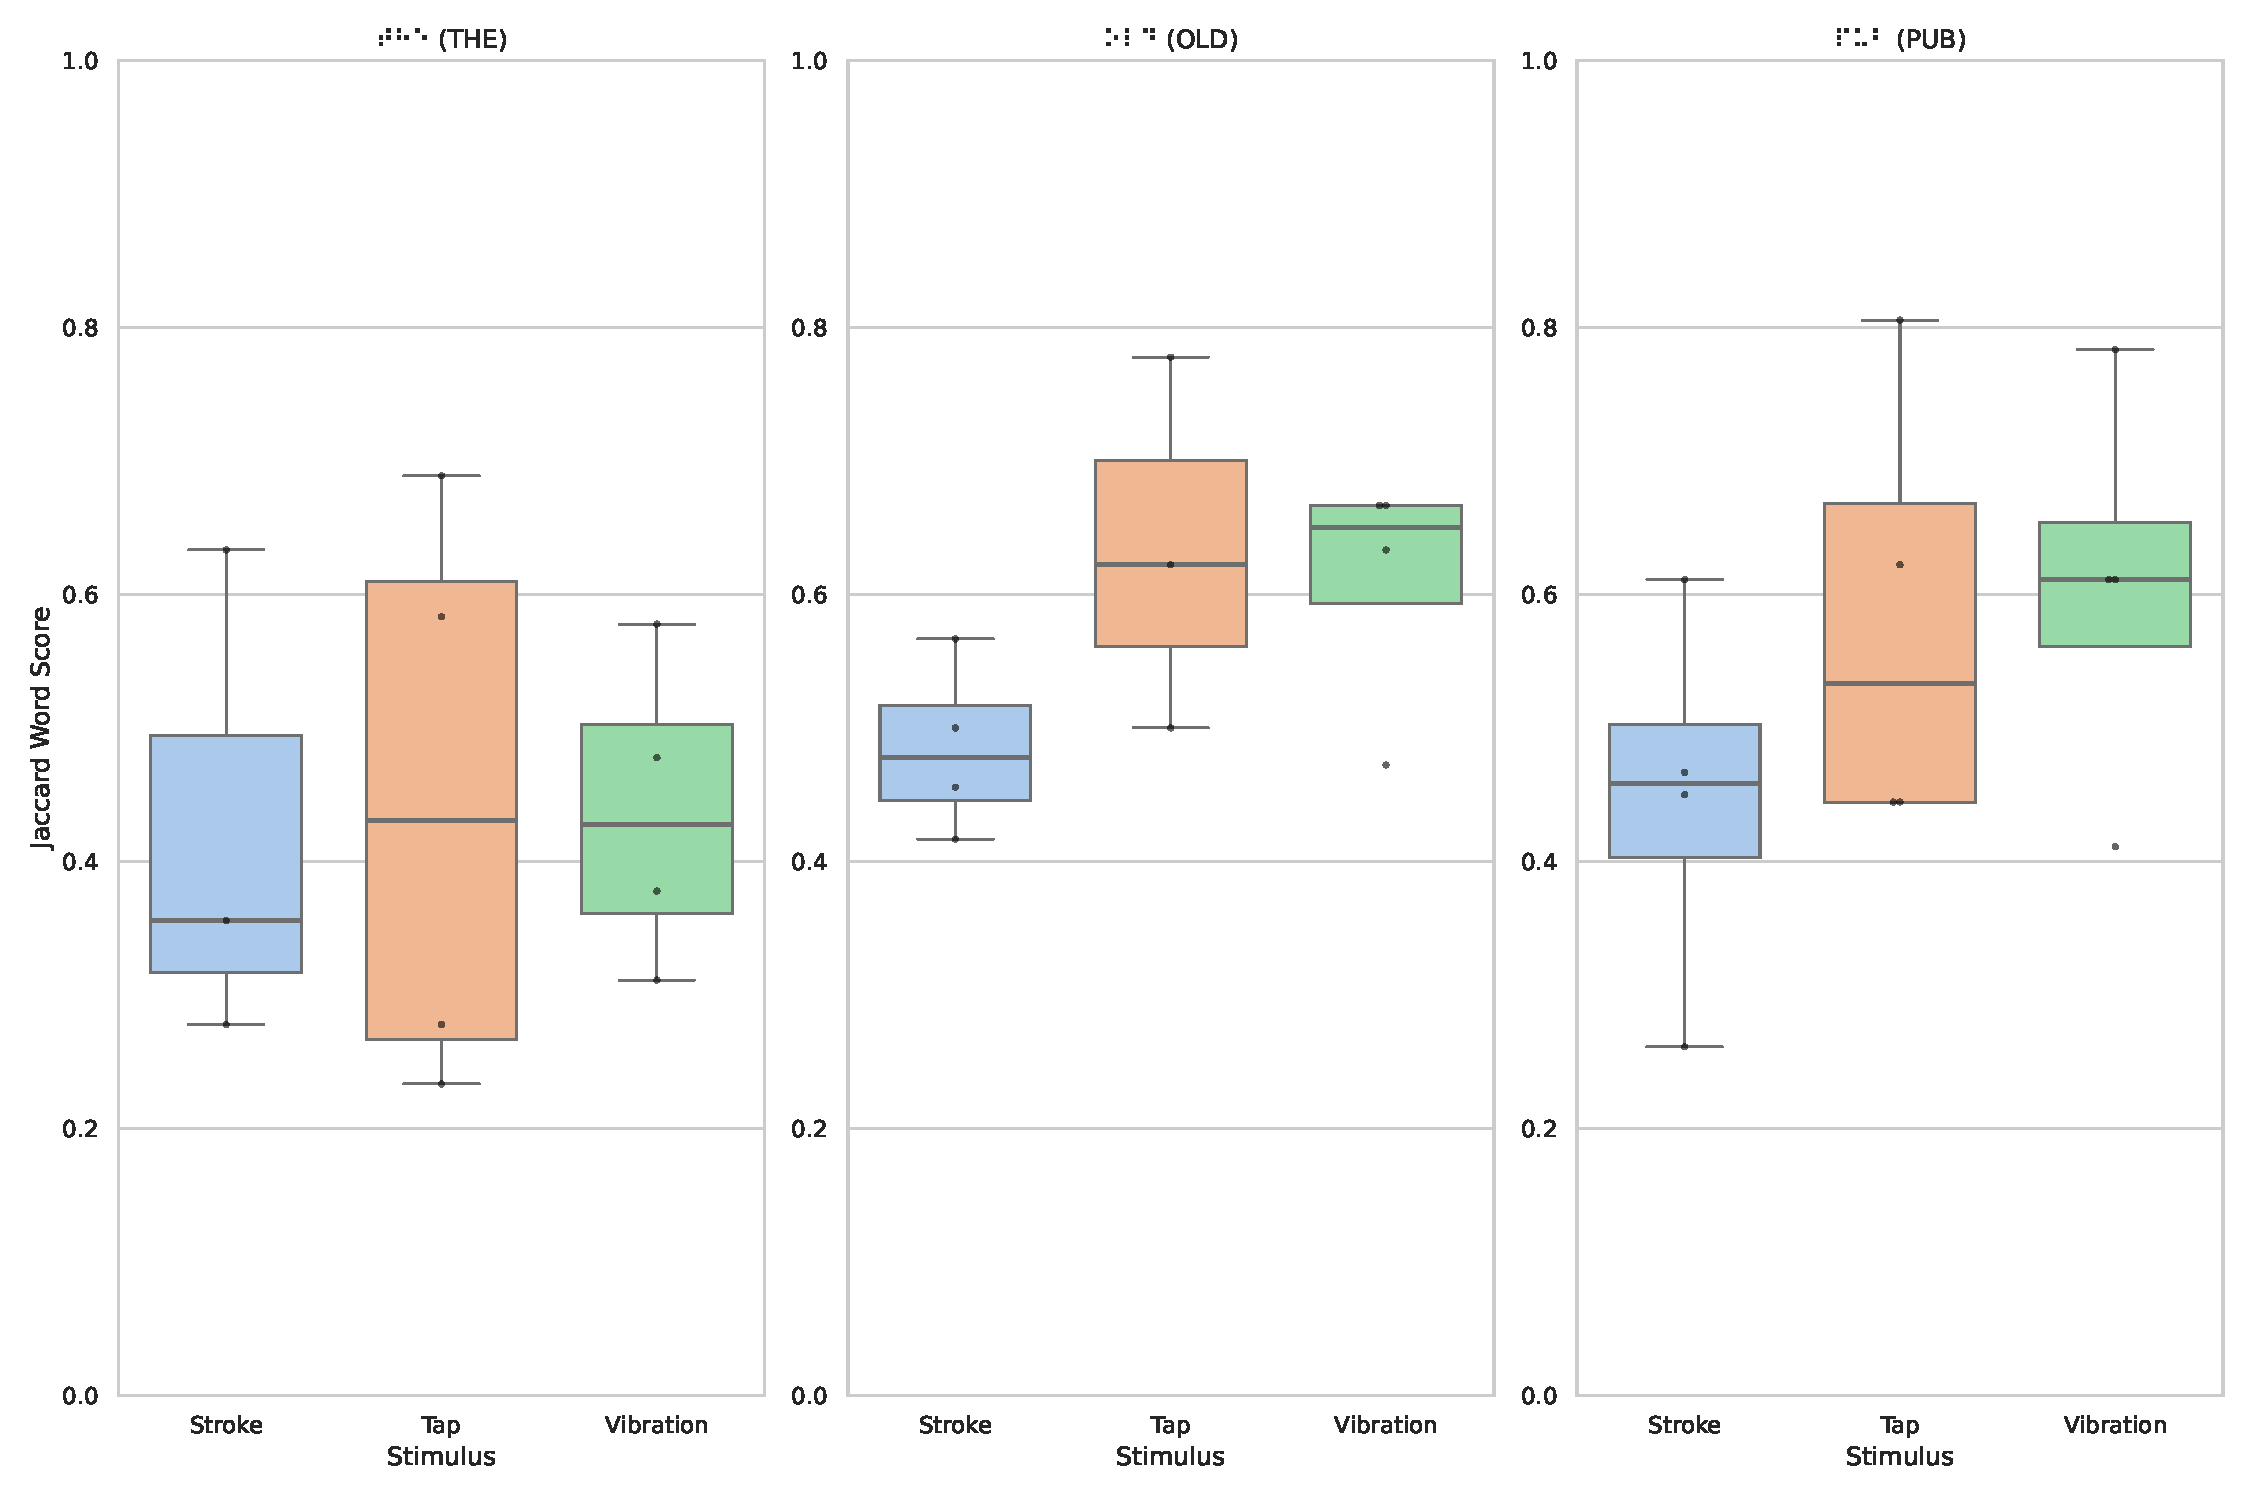
\includegraphics[width=\linewidth]{src/pictures/Study1Data/study1_test_results.pdf}

    
\begin{table}[ht]
\resizebox{\columnwidth}{!}{
\centering
\begin{tabular}{|l|l|l|l|l|}
\hline
\textbf{Question} & \textbf{Test Statistic} & \textbf{p-value}  &\textbf{Significance}           &\textbf{Effect Size}\\ \hline
\braille{the}(\textbf{THE})& 0.0361& 0.9821&Not Significant &0.0036\\ \hline
\braille{old}(\textbf{OLD})& 3.9736 & 0.1371  &Not Significant &0.1371\\ \hline
\braille{pub}(\textbf{PUB})& 1.0569& 0.5895&Not Significant &0.0961\\ \hline
\end{tabular}}
\caption{Results of the Kruskal-Wallis significance tests for the wordtests \enquote{THE}, \enquote{OLD}, and \enquote{PUB} with a $\eta^2$ Effect Size.}
\label{table:significance_results_test_firstStudy}
\end{table}
stroking worse for all of them
Vibration slighlt better than tapping


    \item (We analysed those word results for differences between the single characters)
        
        \centering
        \includegraphics[width=\linewidth]{src/pictures/Study1Data/character_f1_test_study1.pdf}


\begin{table}[ht]
\resizebox{\columnwidth}{!}{
\centering
\begin{tabular}{|l|l|l|l|l|}
\hline
\textbf{Question} & \textbf{Test Statistic} & \textbf{p-value}  &\textbf{Significance}           &\textbf{Effect Size}\\ \hline
\braille{t}(\textbf{T})& 1.0203& 0.6004&Not Significant &0.1131\\ \hline
\braille{h}(\textbf{H})& 0.0136& 0.9932&Not Significant &0.0017\\ \hline
\braille{e}(\textbf{E})& 0.0979& 0.9522&Not Significant &0.0121\\ \hline
\braille{o}(\textbf{O})& 0.5309& 0.7669&Not Significant &0.0622\\ \hline
\braille{l}(\textbf{L})& 3.3764& 0.1849&Not Significant &0.2968\\ \hline
\braille{d}(\textbf{D})& 0.5290& 0.7676&Not Significant &0.0620\\ \hline
\braille{p}(\textbf{P})& 1.6124& 0.4465&Not Significant &0.1519\\ \hline
\braille{u}(\textbf{U})& 2.5488& 0.2796&Not Significant &0.2207\\ \hline
\braille{b}(\textbf{B})& 5.7683& 0.0559&Not Significant &0.3906\\ \hline
\end{tabular}}
\caption{Results of Kruskal-Wallis significance tests for the different Braille characters during testing with a $\eta^2$ Effect Size.}
\label{table:learning_significance_results_firstStudy_nonParam}
\end{table}
L, U
L = tap best, no errors
h,p stroking slightly better otherwise worse
vibration mostly like Tap, but worse for P, D,H
B = difference between strok, vibration big, tap 2nd best


    \item (We analysed the total errors in the test-Words)

    \centering
    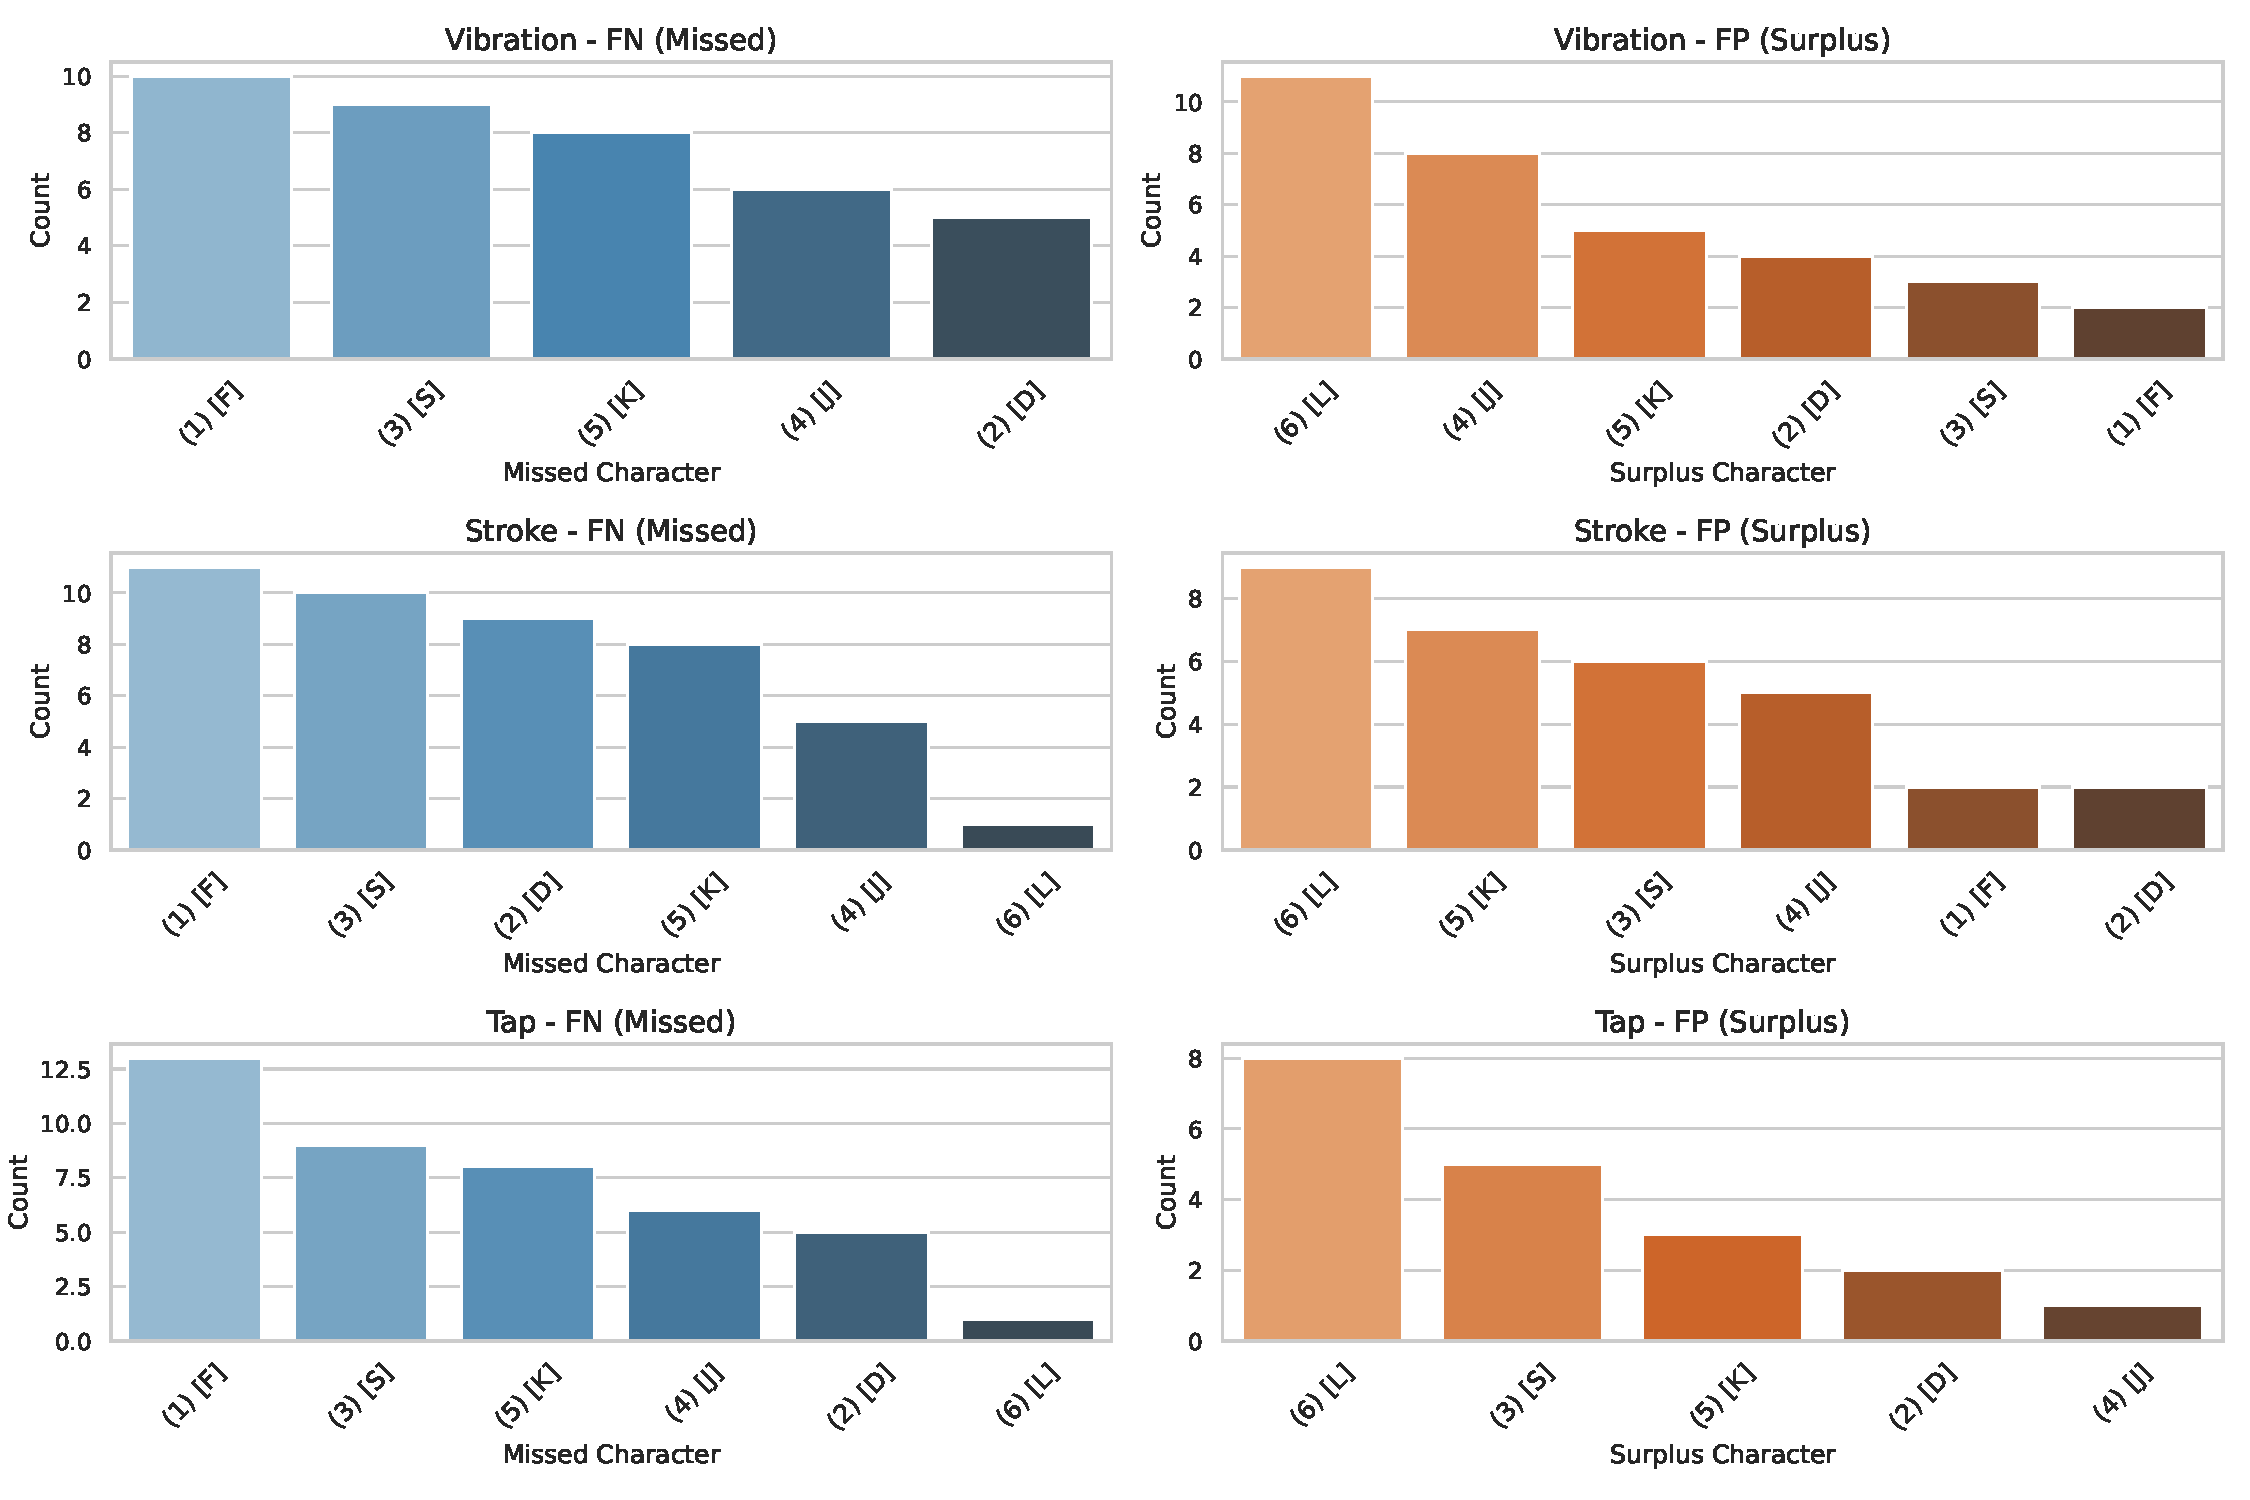
\includegraphics[width=\linewidth]{src/pictures/Study1Data/missed_surplus_test_study1.pdf}


F,S,K,(D) are the most FN (D for stroking)
D[2],J[4] are mostly not missed (except stroking)

L[6] added too often FP
F[1] least FP

    \item (We analysed the errors given a Braille Character from the test-words)
    

        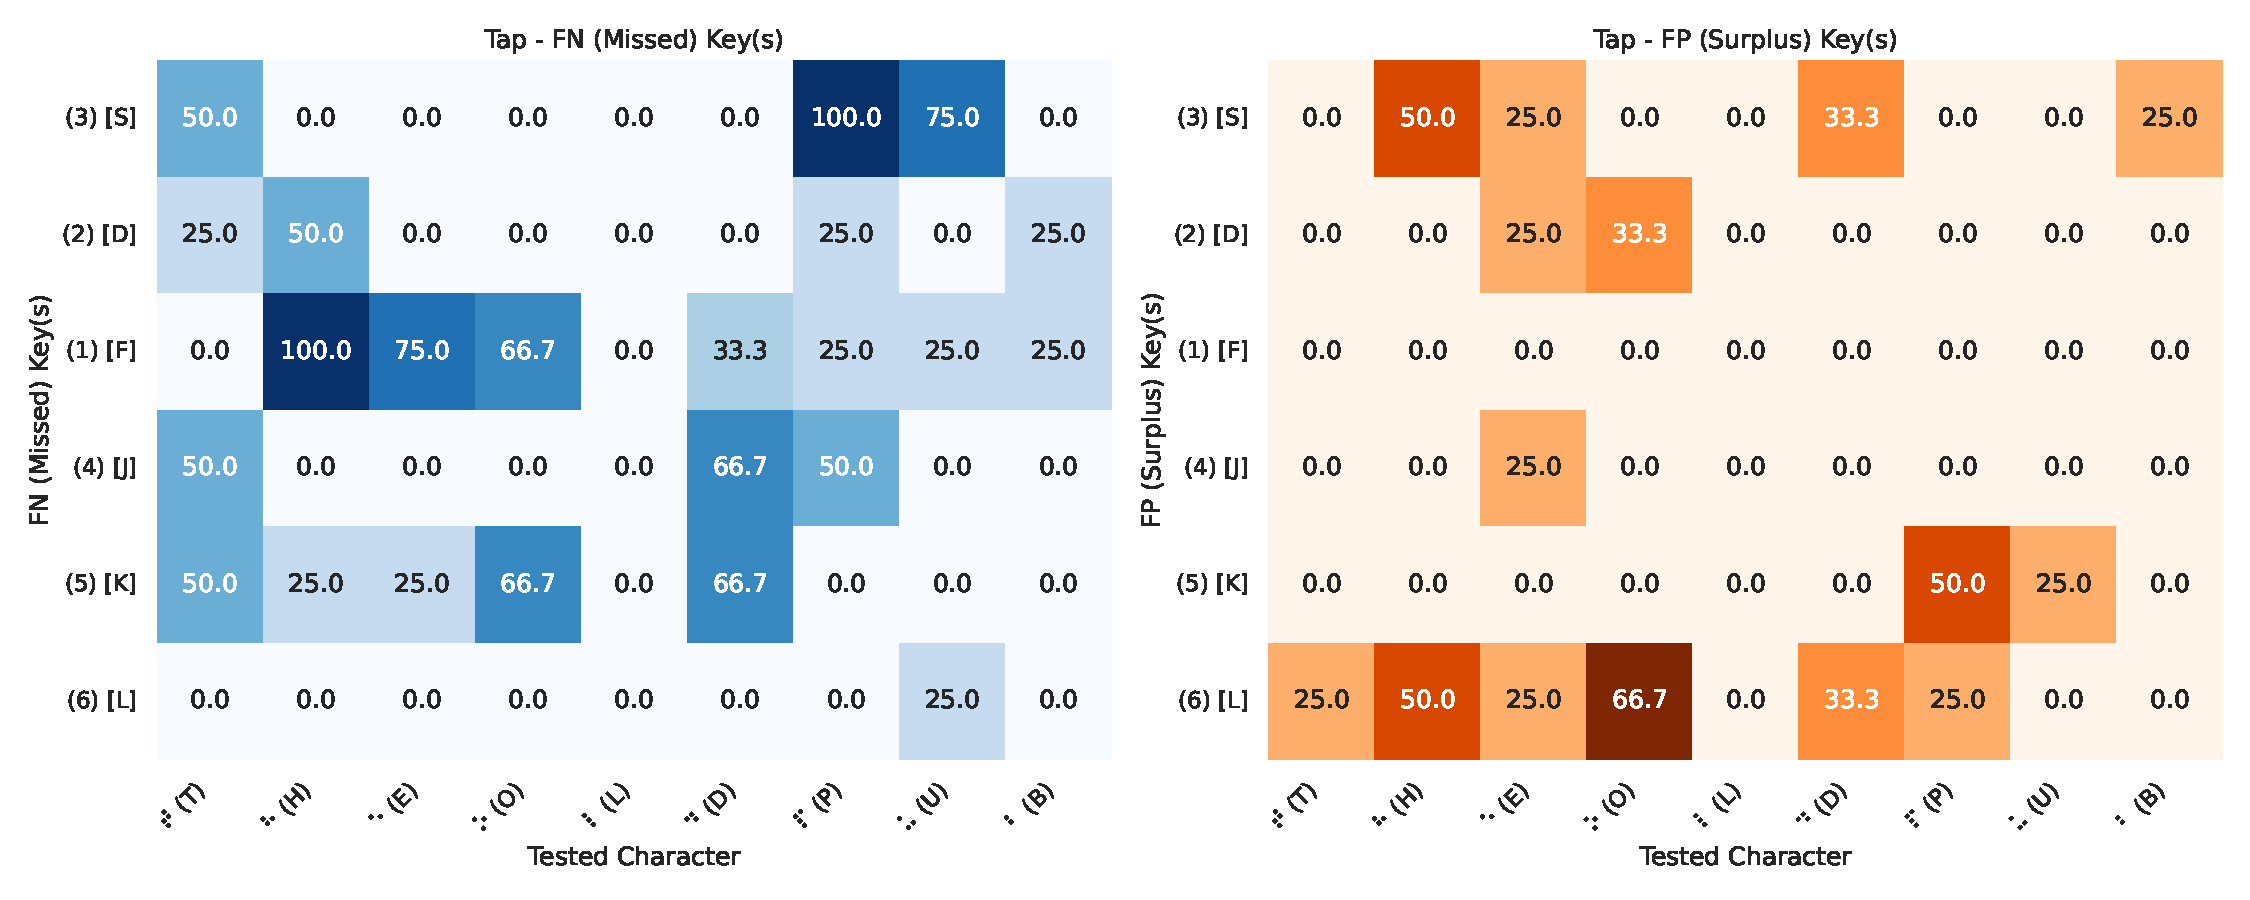
\includegraphics[width=\textwidth]{src/pictures/Study1Data/missed_surplus_test_percentages_study1_T.pdf}
Tap:
S[3] was missed more than 50\% all the times it needed to be pressed, same for the J[4]
All characters composing the braille L (\braille{l}) were found all the time
L and S were often pressed for the braille H even though it is wrong

        
        \centering
        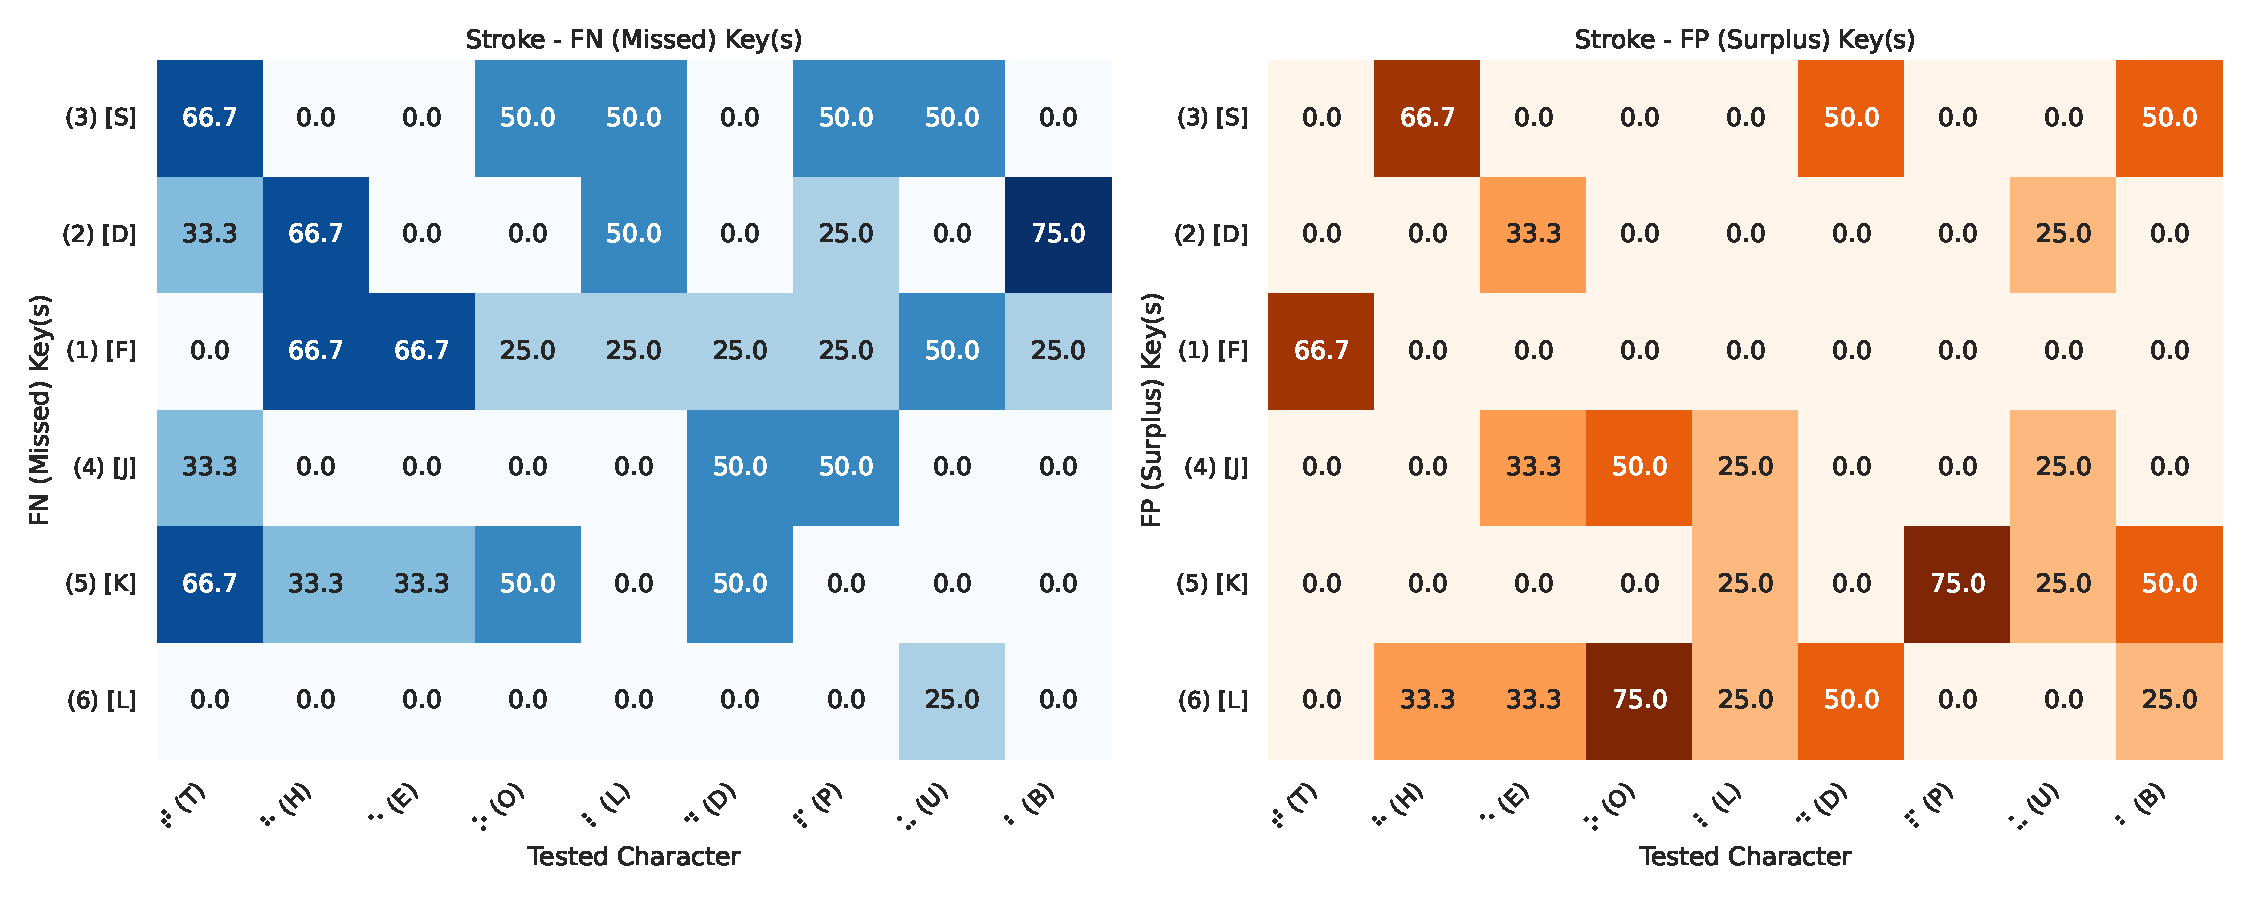
\includegraphics[width=\textwidth]{src/pictures/Study1Data/missed_surplus_test_percentages_study1_S.pdf}
Stroke:
The S[3] was also missed in most of the cases, however compared to the tapping there was no key missed all the time, nevertheless the L wasn't error free as with the tapping one.
The braille L \braille{L}



        \centering
        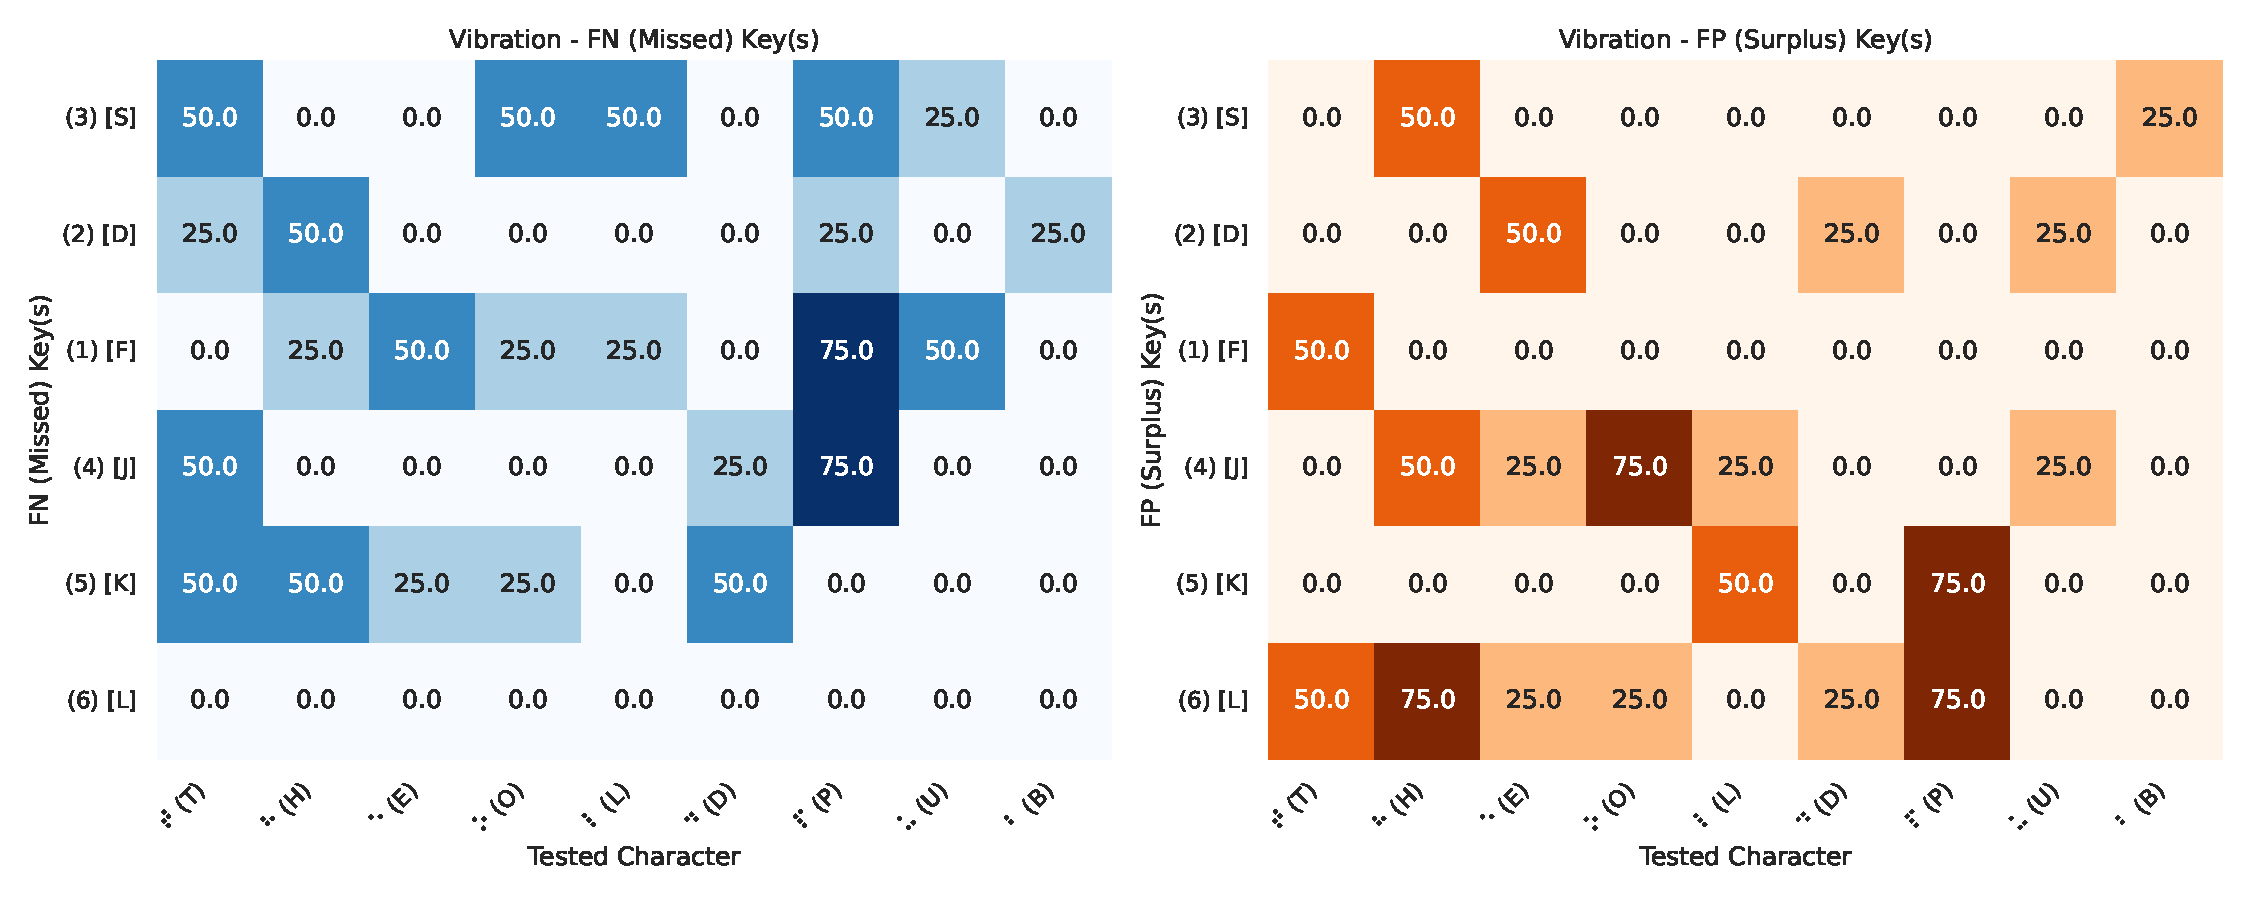
\includegraphics[width=\textwidth]{src/pictures/Study1Data/missed_surplus_test_percentages_study1_V.pdf}
Vibration:
The L[6] key was never missed when it needed to be pressed, however it was pressed too often when it didn't needed to be pressed, similar to the other simuli.

    \item (In order to see the largest error-difference for the characters more visually appealing and using a cosine Similarity as it is comon in NLP word comparissons we plotted the PCA plots.)
    
    \centering
    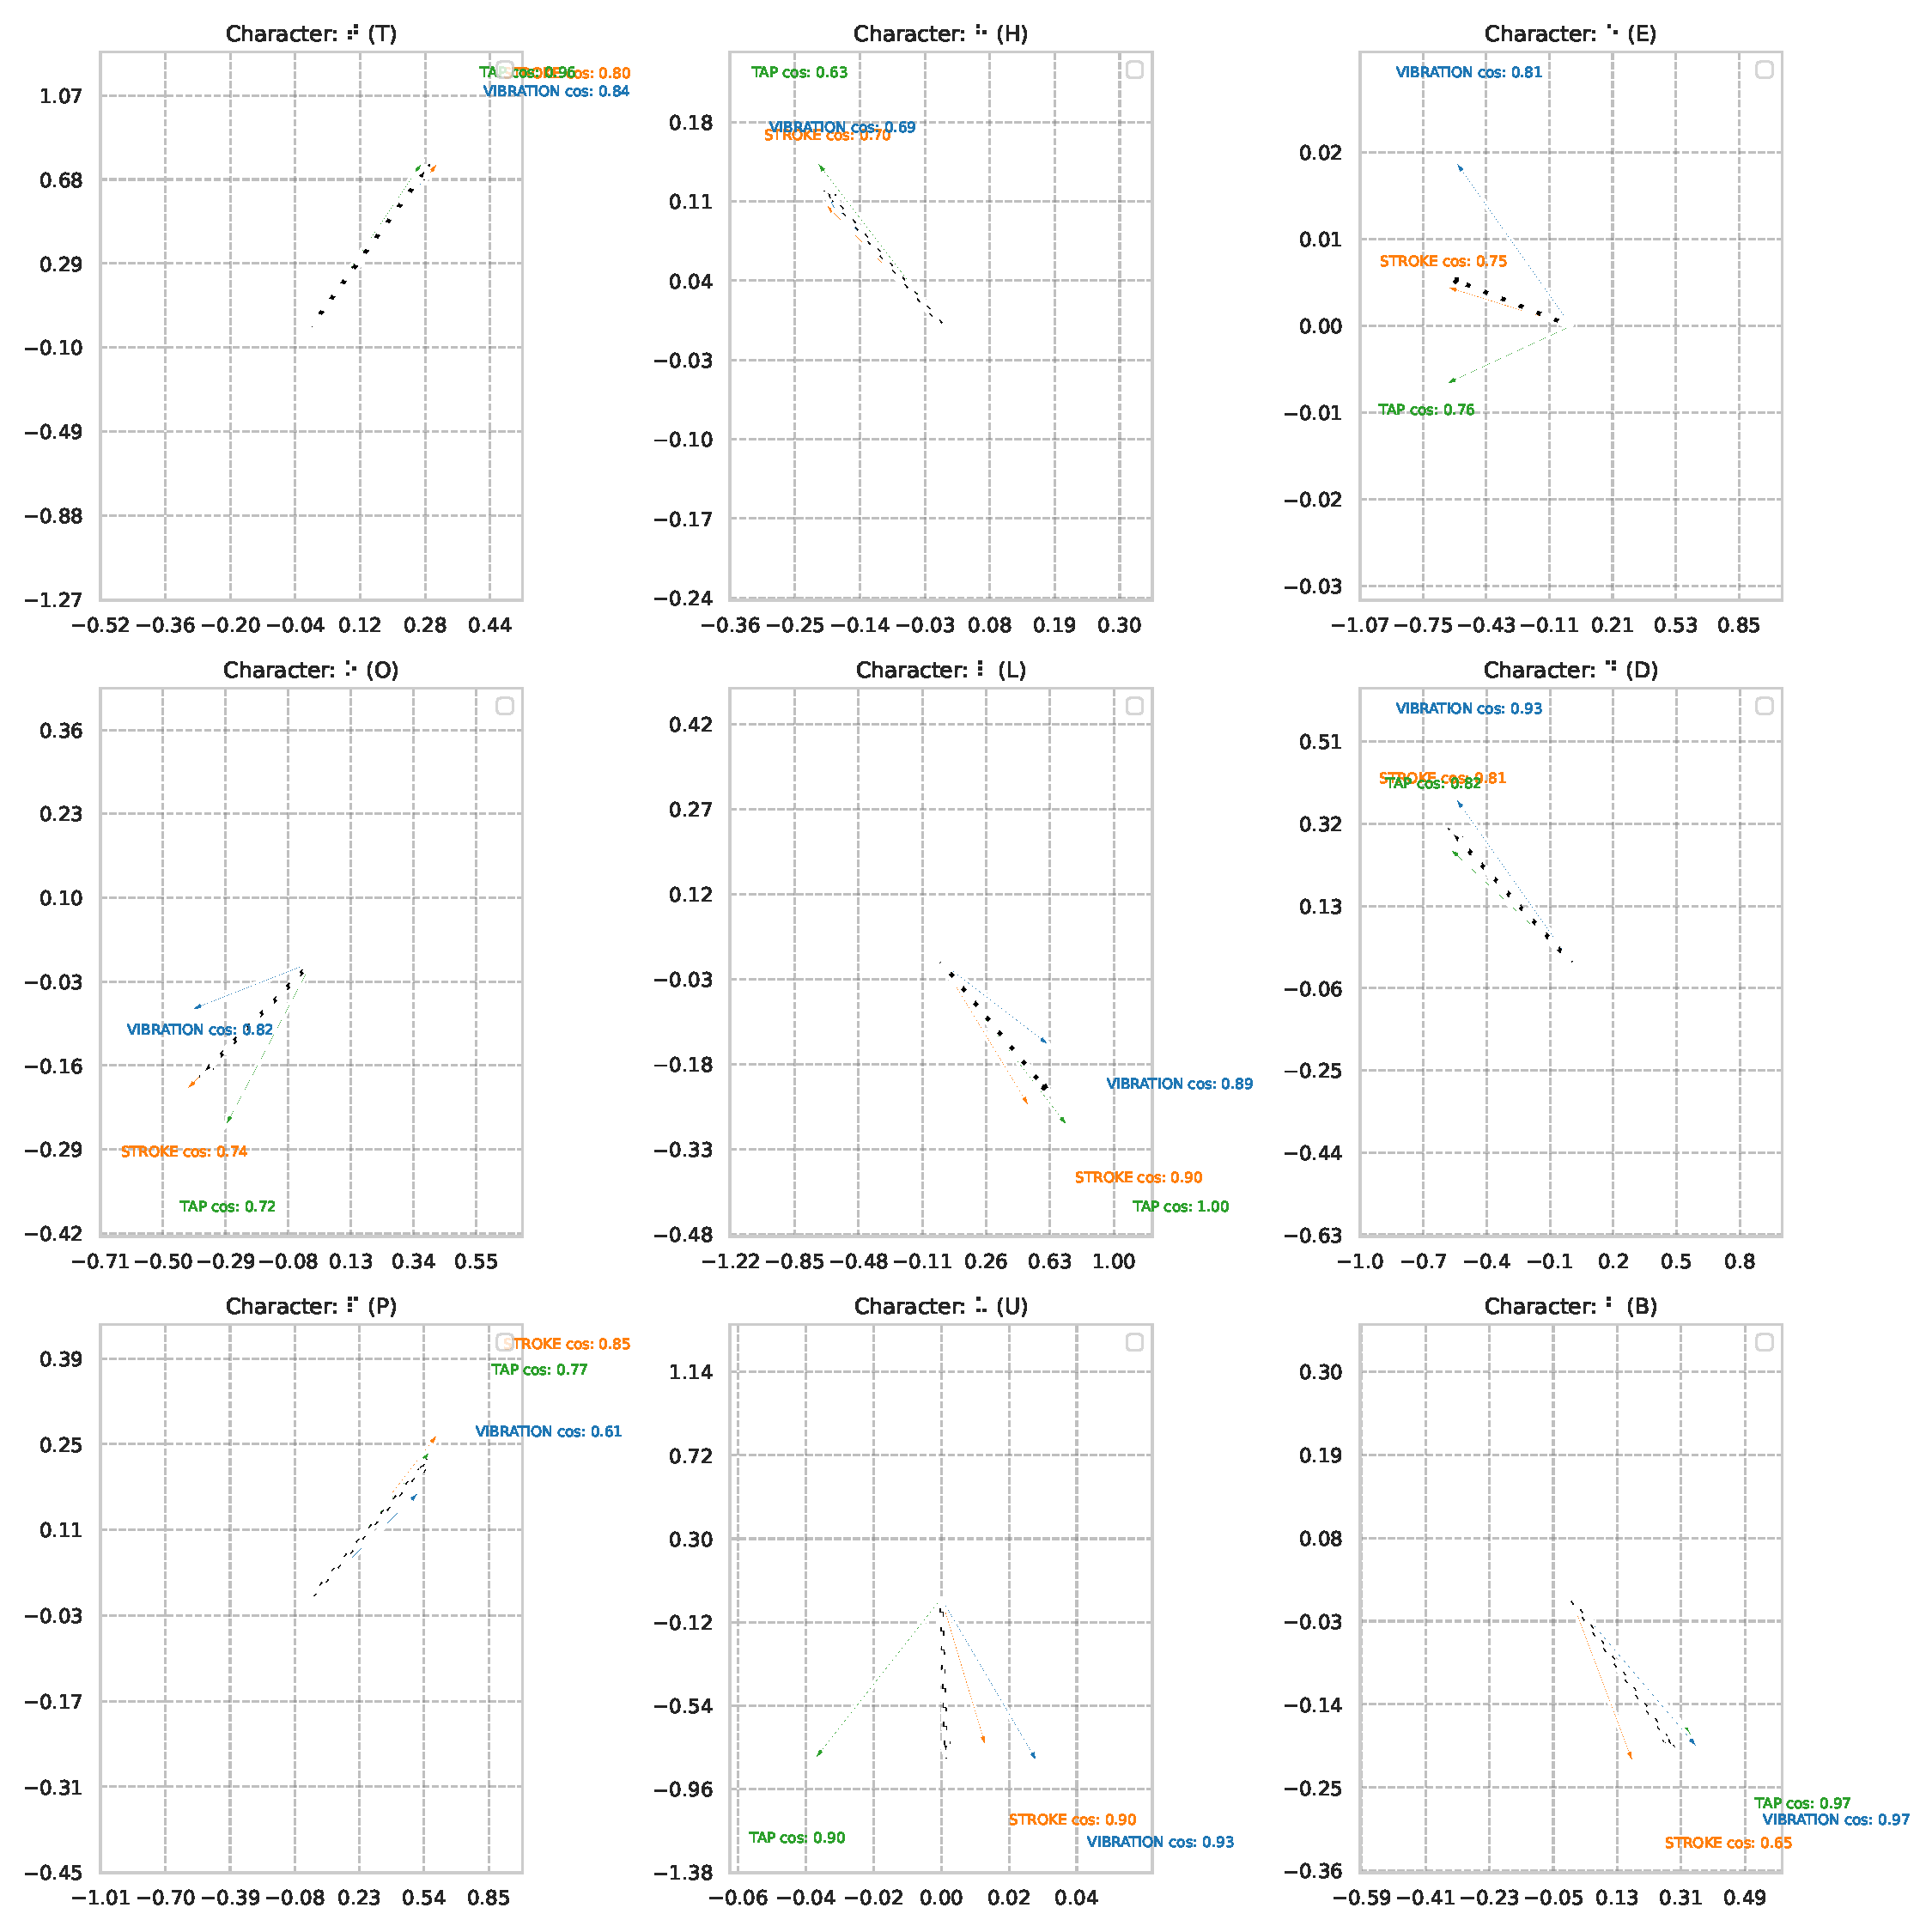
\includegraphics[width=\linewidth]{src/pictures/Study1Data/Vectors_study1.pdf}
This diagram is used to visualise the errors in the previous diagrams better and compare them by splitting it into the dimension with the most differences.
However the show, that most of the data is similar.
Also comparing their cosine similarity yielded, that there are no significant differences.

    \item After passively Learning with a stimulus we conducted a NASA TLX for the task-load
    
        \centering
        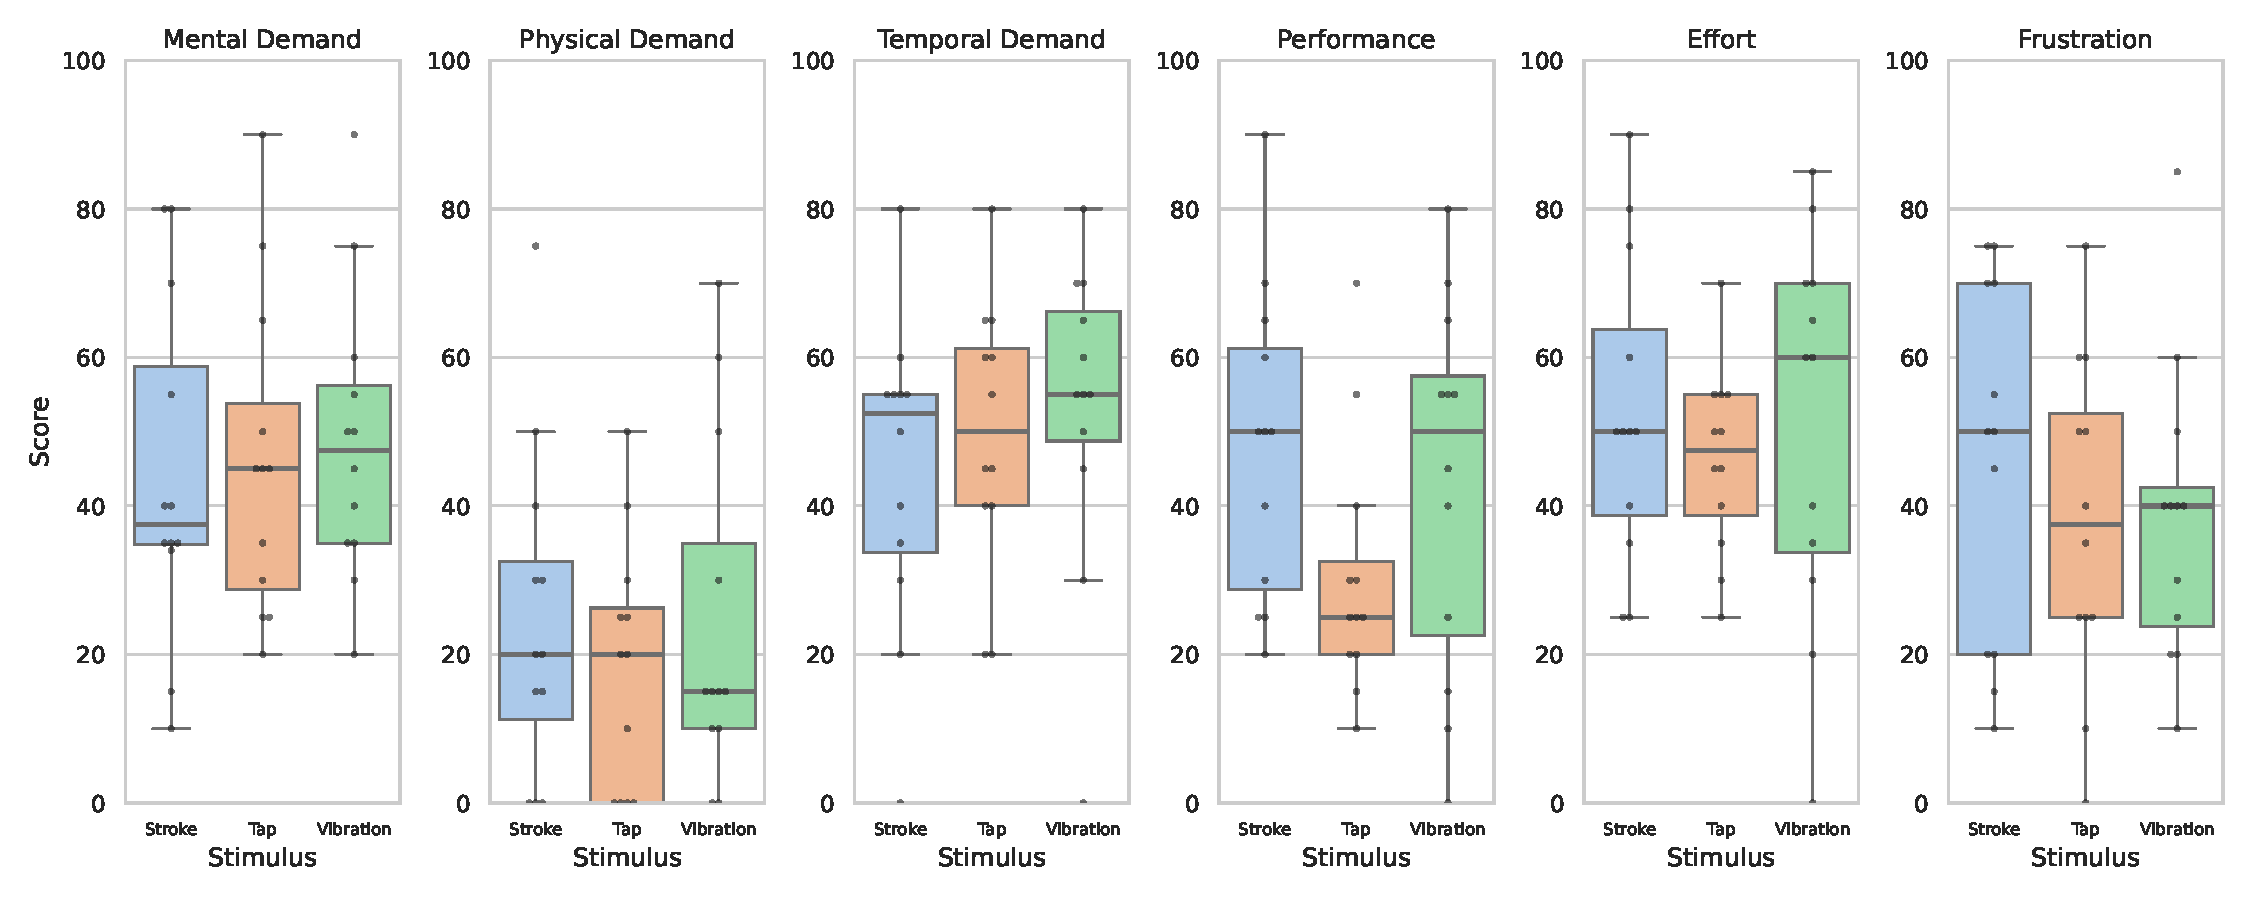
\includegraphics[width=\linewidth]{src/pictures/Study1Data/NasaTLX_study1.pdf}


\begin{table}[ht]
\resizebox{\columnwidth}{!}{
\centering
\begin{tabular}{|l|l|l|l|l|}
\hline
\textbf{Question}        & \textbf{H-Statistic}& \textbf{p-value}       & \textbf{Significance}           &\textbf{Effect Size}\\ \hline
\textbf{Mental Demand}    & 0.5311& 0.7668& Not Significant                 &0.0152\\ \hline
\textbf{Physical Demand}  & 0.358& 0.8361                 & Not Significant                 &0.0102\\ \hline
\textbf{Temporal Demand}  & 1.6356& 0.4414& Not Significant                 &0.0467\\ \hline
\textbf{Performance}      & 3.7994& 0.1496& Not Significant                 &0.1086\\ \hline
\textbf{Effort}           & 0.7655& 0.6820& Not Significant                 &0.0219\\ \hline
\textbf{Frustration}      & 0.9098& 0.6345& Not Significant                 &0.0260\\ \hline
\end{tabular}}
\caption{Results of the Kruskal-Wallis significance tests for the different NasaTLX dimensions with a $\eta^2$ Effect Size.}
\label{table:nasaTLX_significance_firstStudy_nonParam}
\end{table}

    \item Also we conducted asked the participants to rate the usefulness and satisfaction about the current Stimulus
    
        \centering
        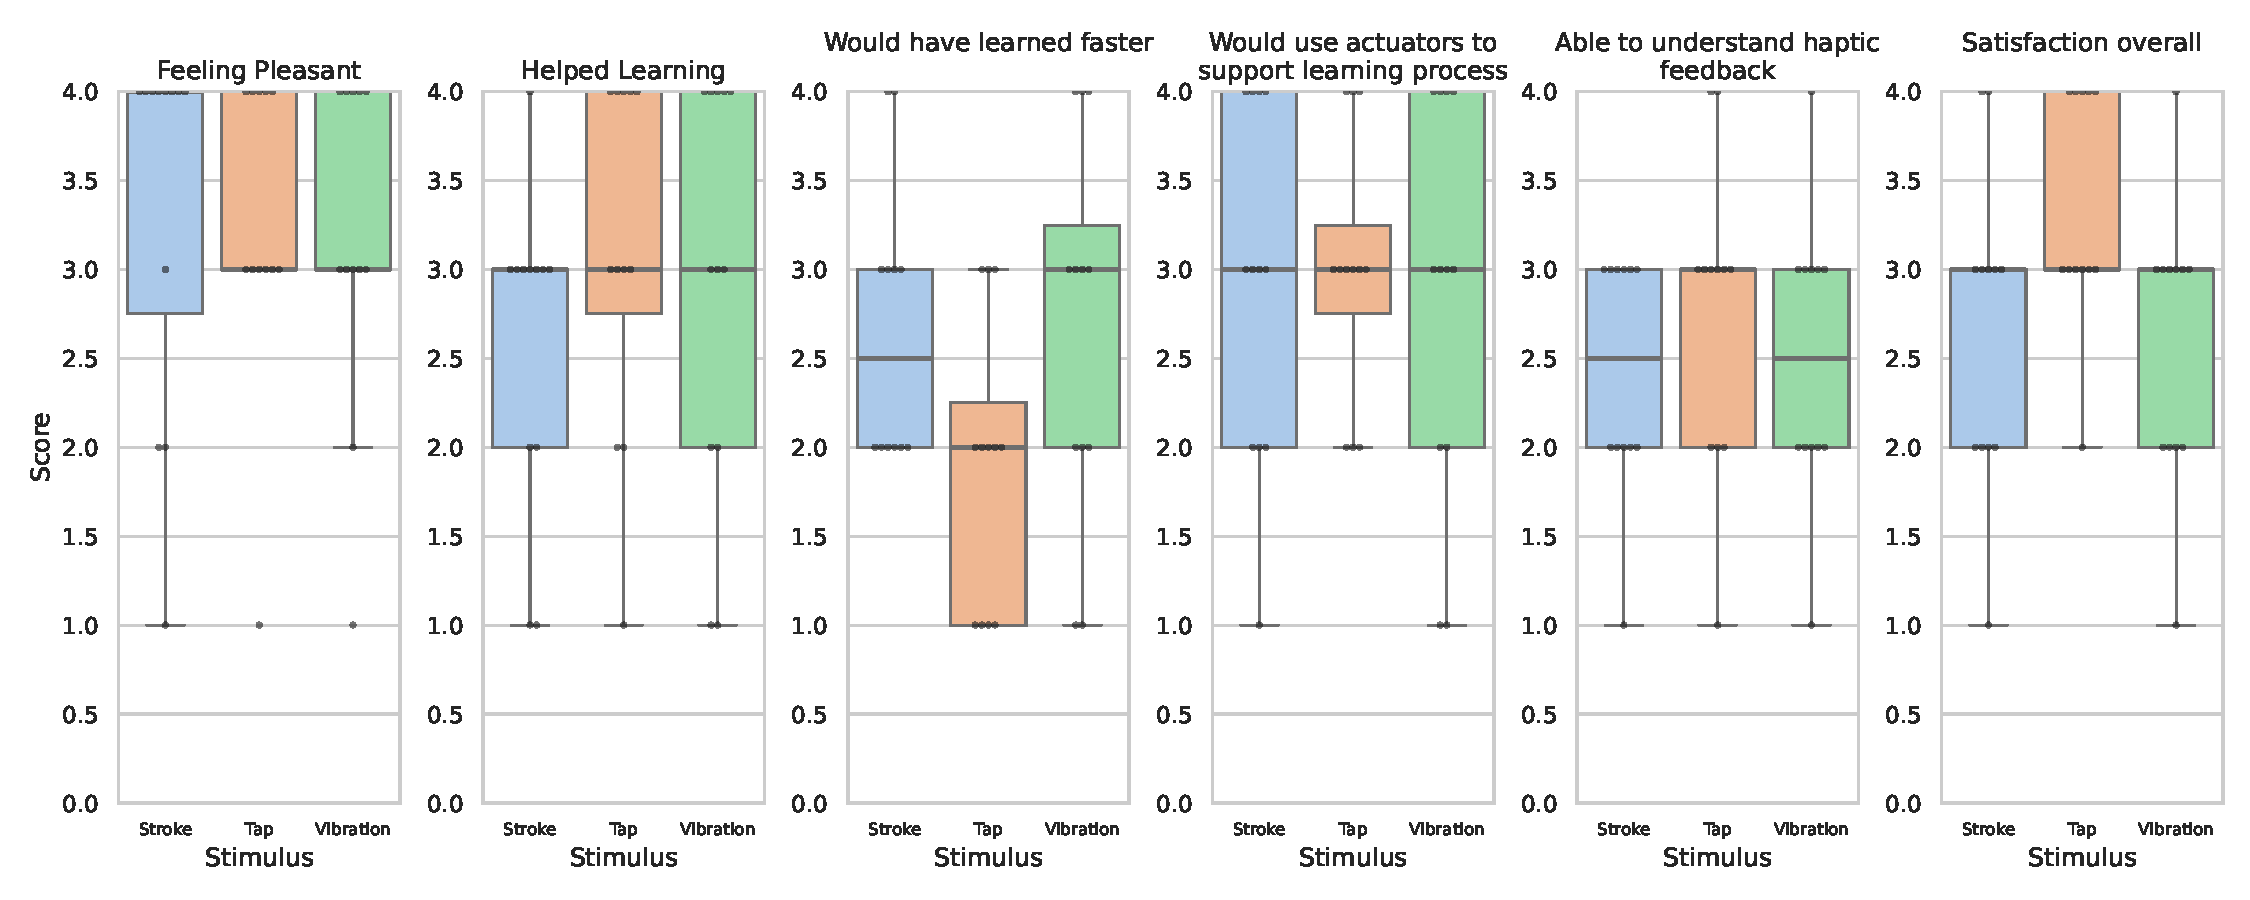
\includegraphics[width=\linewidth]{src/pictures/Study1Data/questions_special_study1.pdf}
 
\begin{table}[ht]
\resizebox{\columnwidth}{!}{
\centering
\begin{tabular}{|l|l|l|l|l|}
\hline
\textbf{Question}                              & \textbf{H-statistic}& \textbf{p-value}       & \textbf{Significance}           &\textbf{Effect Size}\\ \hline
\textbf{Feeling Pleasant}                      & 0.706& 0.7026                 & Not Significant                 &0.0202\\ \hline
\textbf{Helped Learning}                       & 1.942& 0.3787                 & Not Significant                 &0.0555\\ \hline
\textbf{Would have learned faster}             & 4.855& 0.0882                 & Not Significant                 &0.1387\\ \hline
\textbf{Would use actuators to support learning process} & 0.038& 0.9812                 & Not Significant                 &0.0011\\ \hline
\textbf{Able to understand haptic feedback}    & 1.241& 0.5377                 & Not Significant                 &0.0355\\ \hline
\textbf{Satisfaction overall}                  & 5.975& 0.0504                 & Not Significant                 &0.1707\\ \hline
\end{tabular}}
\caption{Results of the Kruskal-Wallis significance tests for the different self-assessment dimensions with a $\eta^2$ Effect Size.}
\label{table:individualQuestions_significance_firstStudy}
\end{table}
sattisfactino best for tapping
tapping bad with learnin
tapping haptic fb best
would have learned faster taooing bad

    \item After conducting \textbf{ALL Experiments}, the participants were asked to compare the Simuli against one another

        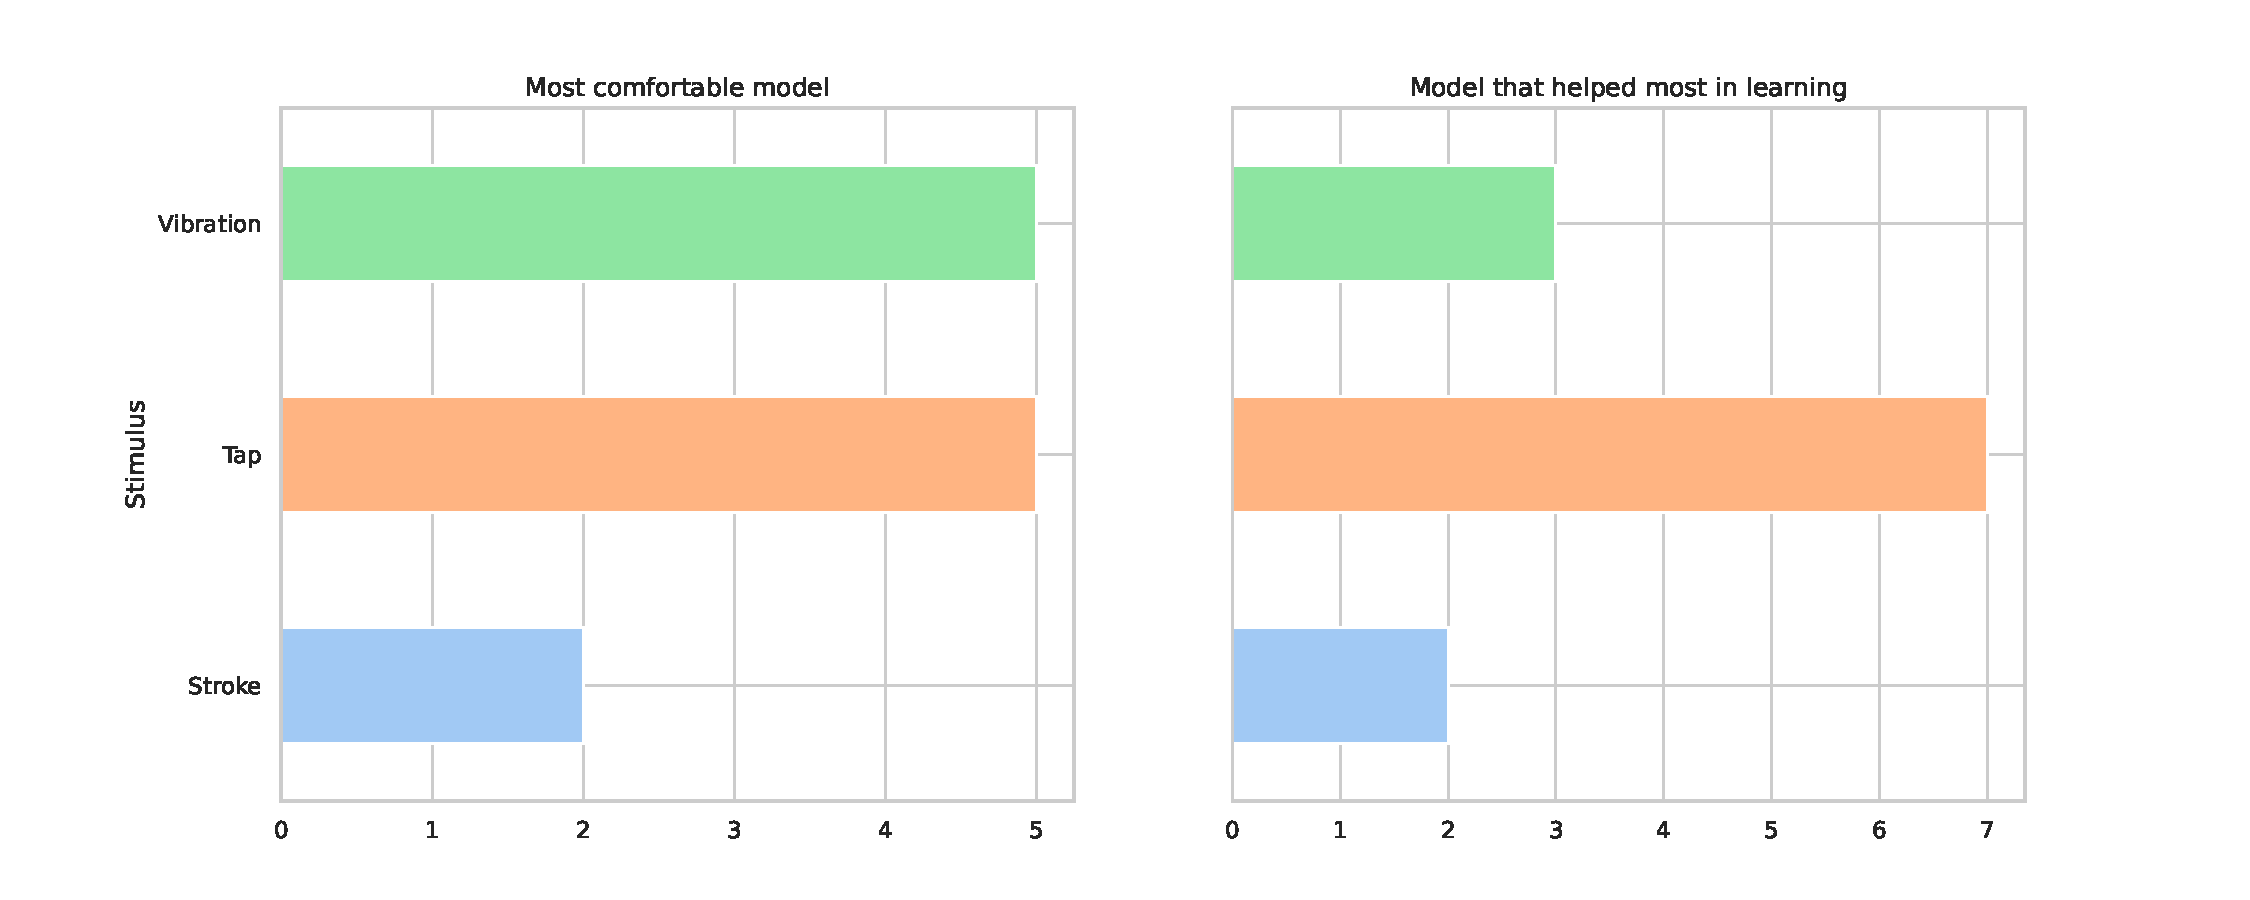
\includegraphics[width=\linewidth]{src/pictures/Study1Data/questions_compare_study1.pdf}

\begin{table}[ht]
\centering
\resizebox{\columnwidth}{!}{
\begin{tabular}{|l|l|l|l|l|}
\hline
\textbf{Question} & \textbf{Test} & \textbf{Test- Statistic}& \textbf{p-value}  &\textbf{Significance}          \\ \hline
Model most comfortable & \gls{csgf}& 1.5 & 0.4724  &Not Significant                \\
 & \gls{emgf}& 3.464*& 0.4568 &Not Significant                \\\hline
Model that helped most in learning & \gls{csgf}& 3.5 & 0.1738 &Not Significant                \\
 & \gls{emgf}& 4.206*& 0.278 &Not Significant                \\\hline
\end{tabular}}
\caption{Statistical Test Results for the direct comparison between the stimuli.\\\text{*} indicates results obtained via Negative Log-Likelihood under $H_0$.}
\label{table:statistical_tests_comparrisson_firstStudy}
\end{table}

direct comparrisson , tappig best, followed by vibration
stroking worse

    \item \textbf{Open Feedback}

    
\begin{table}[H]
\centering
\resizebox{\columnwidth}{!}{
\begin{tabular}{| l |}
\hline
It’s hard to remember the letter while focussing on the game \\
\hline
Stroking is better than Vibration,\\ and Tapping is better than Stoking in both comfortable or learning  \\
\hline
Bei Vibration ist manchmal schwer zu finden, welche Finger vibriert \\
\hline
The game was a bit buggy.\\ The vibration was unclear whether 

some fingers felt the vibration due to other vibrators.\\

The stroke was hard to feel. \\
\hline
Ich empfand den Tapper am angenehmsten und man konnte die finger gut unterscheiden.\\

Den Stroker habe ich manchmal nur kaum gespuert  \\
\hline

\end{tabular}}

\end{table}

\end{enumerate}

tapping best, vibration between fingers hard, same for stroking
stroking perceived different for different ppl

\textbf{Results}

The tapping actuator is the best one due to it being able to distinguish between the fingers, this led to a slightly higher performance than with the other Stimuli.
The vibration is the scond best, however it is hard to distinguish the finger using vibration, as mentinoed in the comments.
The stroker is the worst one, presumably because of the different finger sizes and the stroke not being able to be registered as good by the participant.
We also show that learning using both hands with the ost encoding with affective and discriminative touch is indeed possible.
And we show that tapping is a very good contestant to passive haptic learning instead of using vibration.






\begin{enumerate}
\textbf{RQ2: Is there a significant difference between Learning with a OST Encoding compared to the SEQ one}\\

(General Participant Data)

\resizebox{\columnwidth}{!}{
    \centering
    \begin{tabular}{|c|c|c|c|} \hline 
        Gender & Age & Dominant Hand & Previous Braille Knowledge\\ \hline 
        F & 21 & R & No\\ \hline 
        M & 61 & L & No\\ \hline 
        M & 23 & R & No\\ \hline 
        F & 27 & R & No\\ \hline 
        F & 29 & R & No\\ \hline 
        M & 23 & R & No\\ \hline 
        M & 26 & R & No\\ \hline 
        M & 23 & R & No\\ \hline
    \end{tabular}}

    
(Check the concentration of the participants)

    \centering
    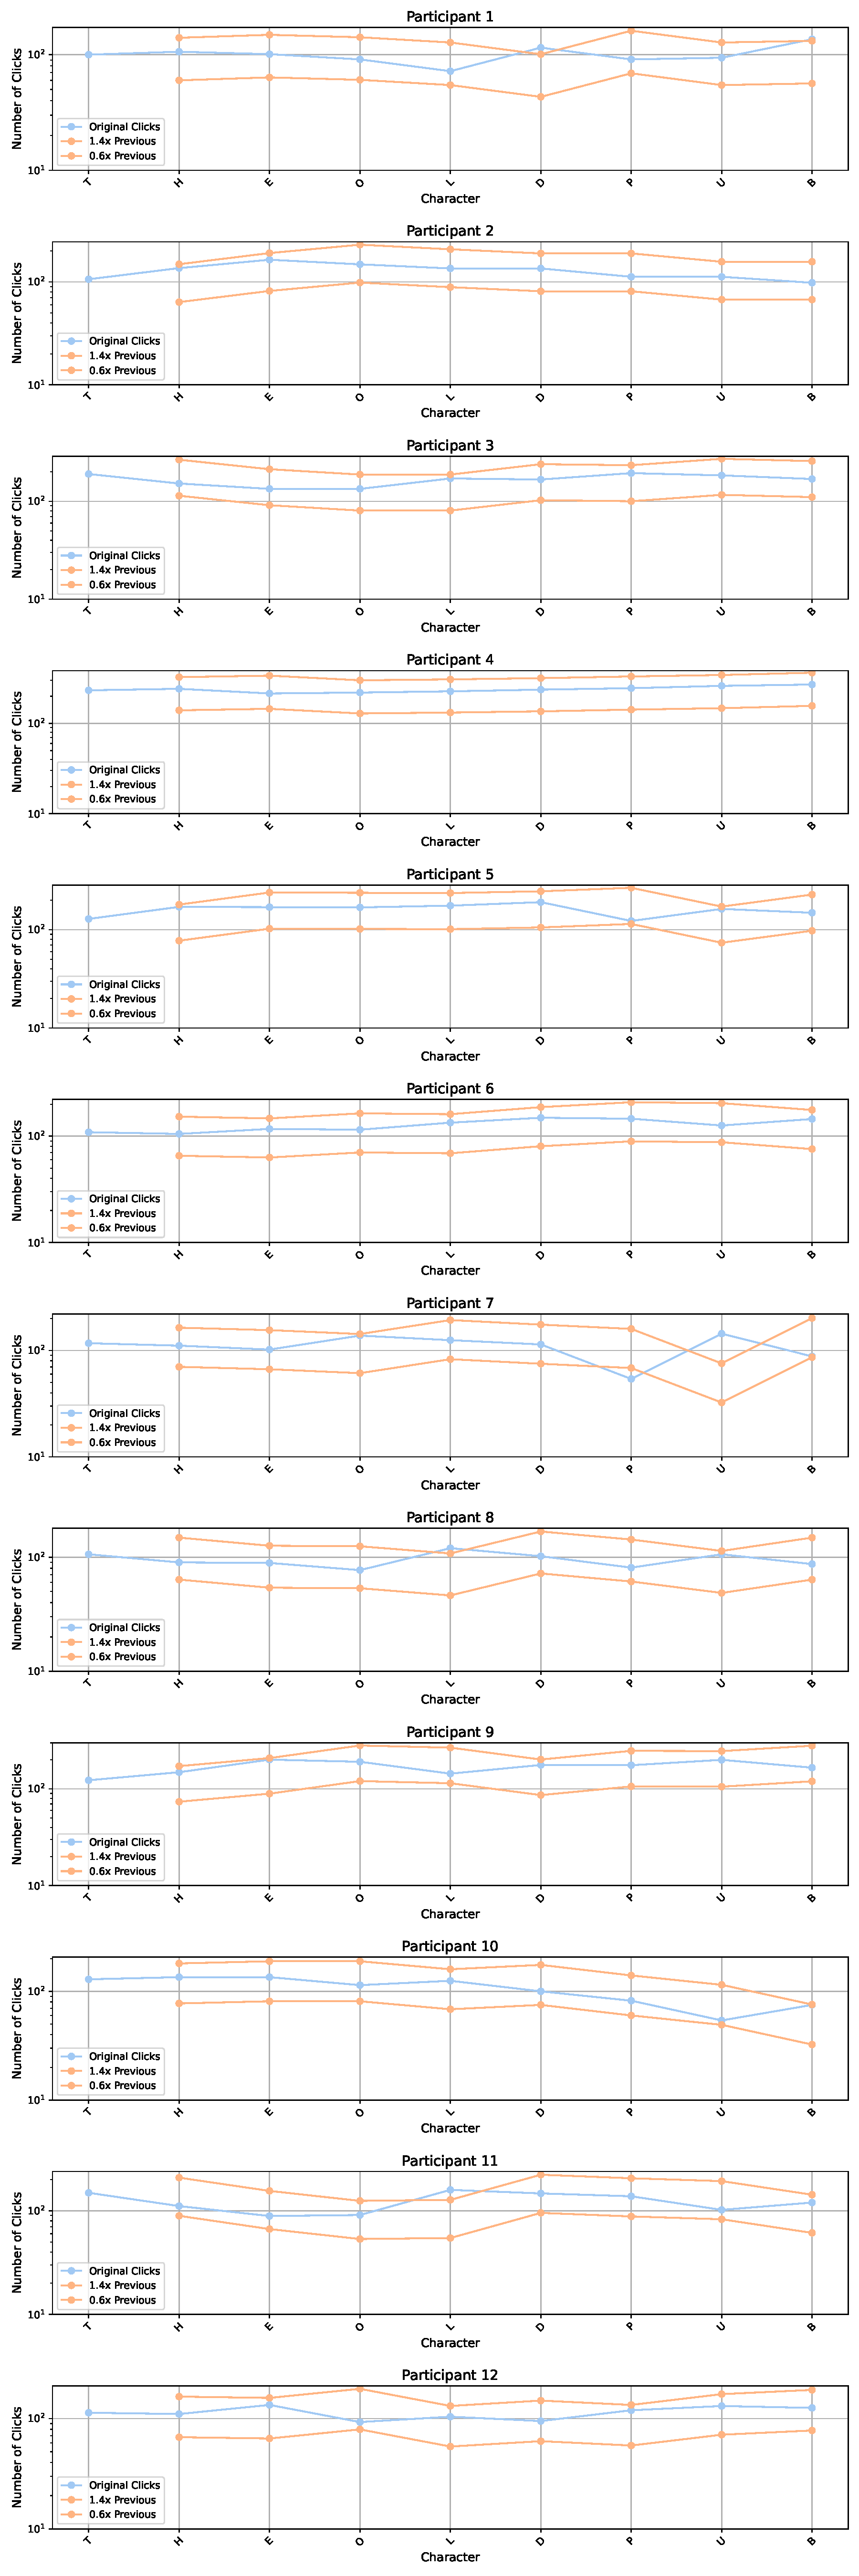
\includegraphics[width=0.5\linewidth]{src/pictures/Study1Data/participantPlots_study1.pdf}




    \item Learning one Braille word consisting out of three Braille characters with one affective/discriminative touch Stimuli passively (\braille{o} (O),\braille{l} (L),\braille{d} (D), \braille{p} (P), \braille{u} (U),\braille{b} (B)) with a test after each character.

    \centering
    \includegraphics[width=\linewidth]{src/pictures/Study2Data/character_f1_test_study2.pdf}

\begin{table}[ht]
\resizebox{\columnwidth}{!}{
\centering
\begin{tabular}{|l|l|l|l|l|}
\hline
\textbf{Question} & \textbf{Test Statistic} & \textbf{p-value}  &\textbf{Significance}           &\textbf{Effect Size}\\ \hline
\braille{o}(\textbf{O})& 10.000& 0.659&Not Significant &0.290\\ \hline
\braille{l}(\textbf{L})& 5.500& 0.552&Not Significant &0.460\\ \hline
\braille{d}(\textbf{D})& 13.500& 0.124&Not Significant &1.424\\ \hline
\braille{p}(\textbf{P})& 14.000& 0.067&Not Significant &1.492\\ \hline
\braille{u}(\textbf{U})& 3.000& 0.180&Not Significant &1.108\\ \hline
\braille{b}(\textbf{B})& 6.000& 0.453&Not Significant &0.707\\ \hline
\end{tabular}}
\caption{Results of the \gls{mwu} and t-test's for significance grouped by the different Braille characters during training for the different Encodings with Cohen's d.}
\label{table:learning_significance_results_secondStudy_nonPar}
\end{table}
seq better for o,d,p = 1,3,5; \textbf{1,4,5}; \textbf{1,2,3,4}
ost better for L,U,B = 1,2,3; \textbf{1,3,6;} \textbf{1,2}
ost better for shorter ones, seq in longer encodings
if there is a "4" involved, or the right hand (except or U), the seq is better

p is almost significant better with seq


    \item After one word was learned with a Stimuli, we conducted a word-tests the Braille word (\braille{THE} (THE), \braille{old} (OLD), \braille{pub} (PUB)).

    \centering
    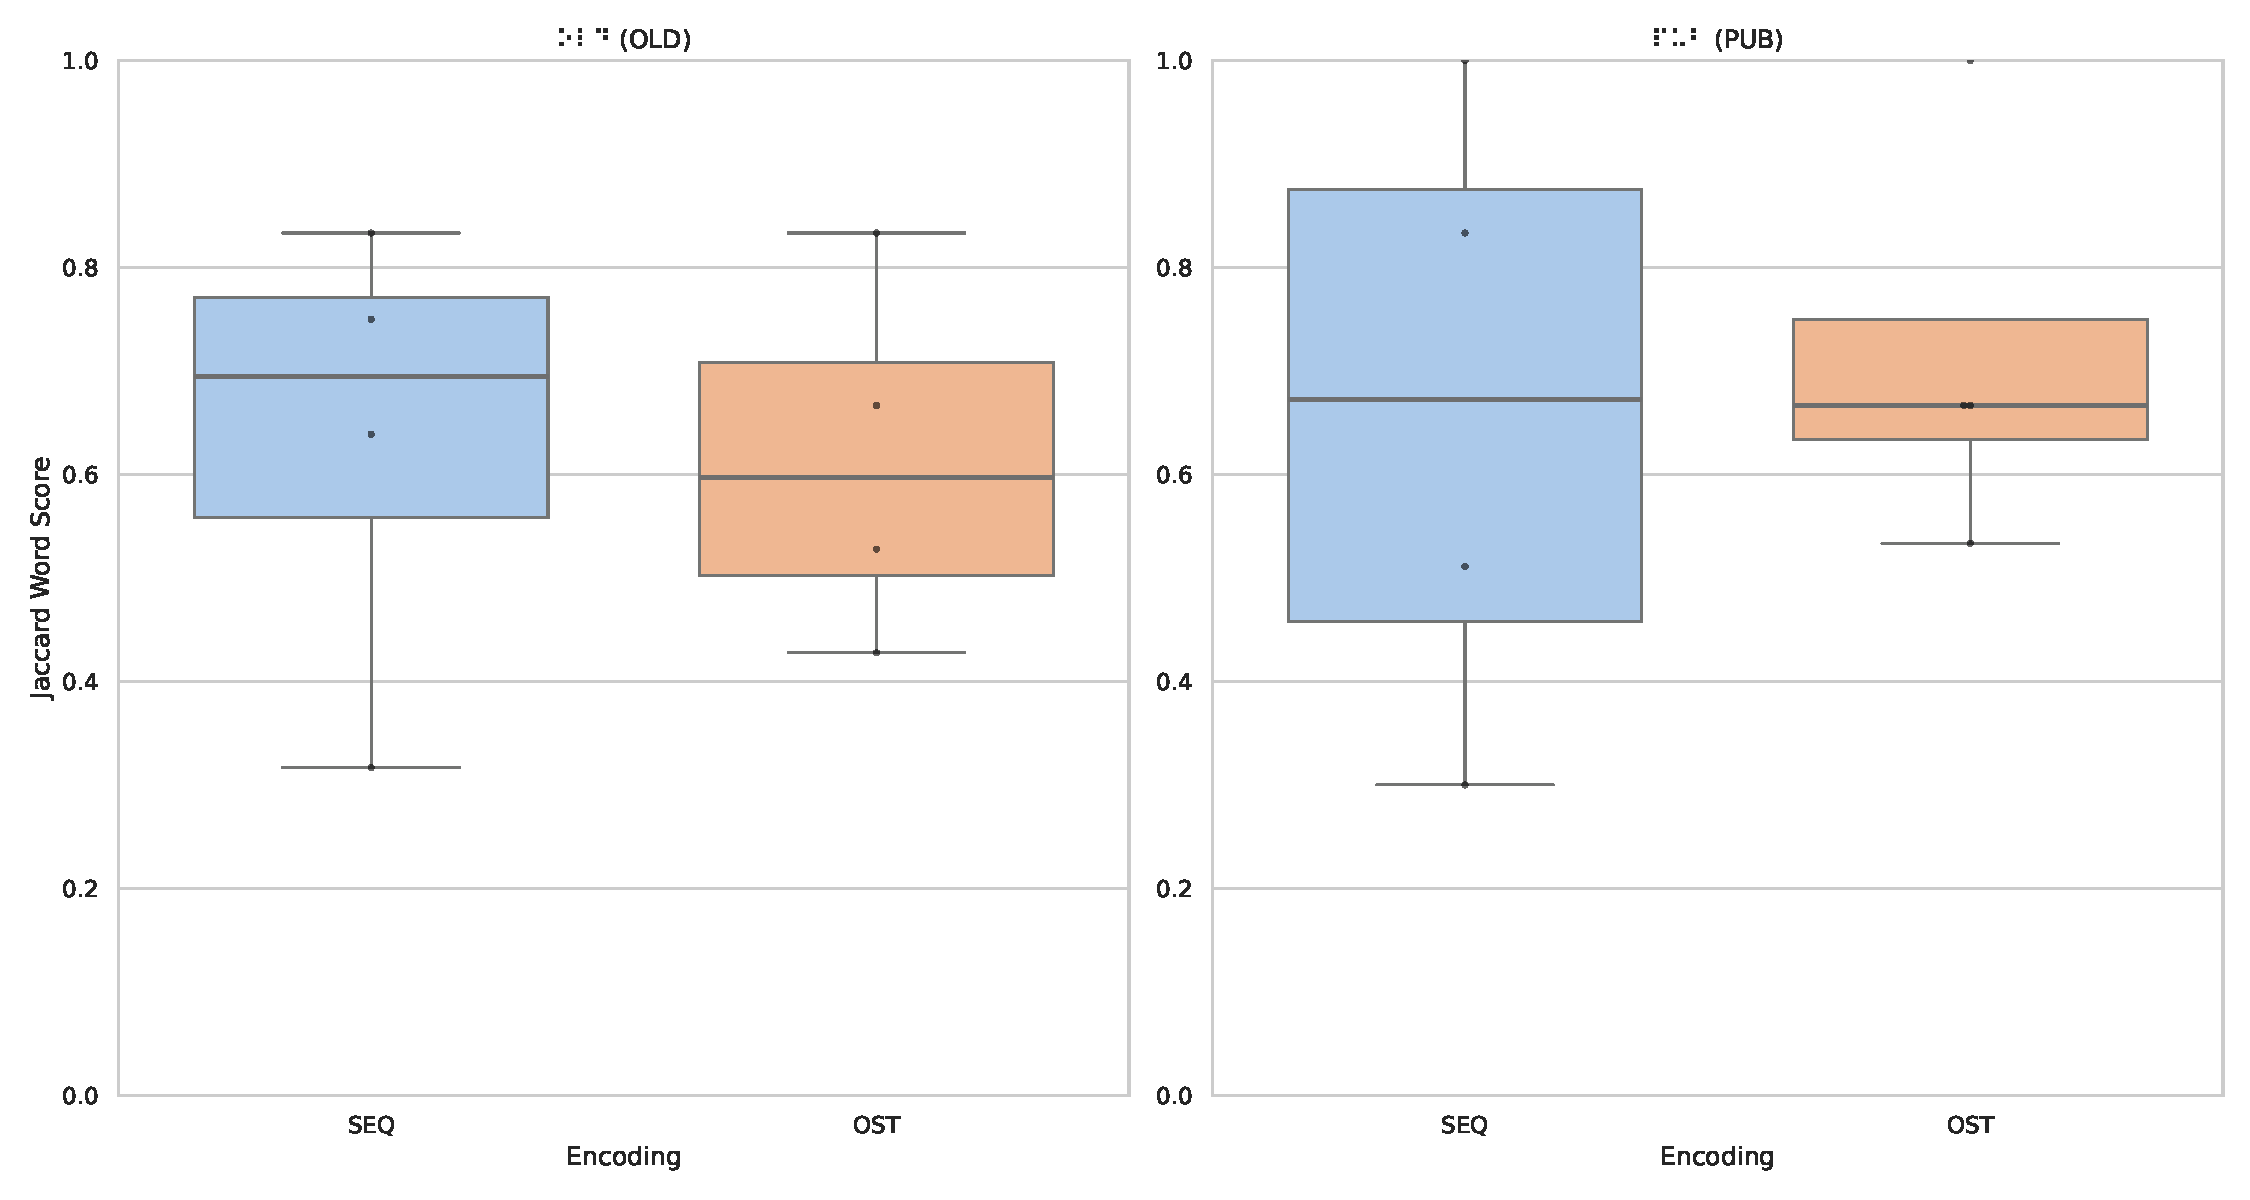
\includegraphics[width=\linewidth]{src/pictures/Study2Data/study2_test_results.pdf}

\begin{table}[ht]
\resizebox{\columnwidth}{!}{
\centering
\begin{tabular}{|l|l|l|l|l|}
\hline
\textbf{Question} & \textbf{Test Statistic} & \textbf{p-value}  &\textbf{Significance}           &\textbf{Effect Size}\\ \hline
\braille{old}(\textbf{OLD})& 8.500& 1.000&Not Significant &0.103\\ \hline
\braille{pub}(\textbf{PUB})& 6.500& 0.770&Not Significant &0.211\\\hline
\end{tabular}}
\caption{Results of the Student t-tests for significance for the different Braille tests-words with a Cohens d Effect Size.}
\label{table:significance_results_test_secondStudy_nonPara}
\end{table}

combination all in all the same, seq slightly better, but has higher variance


    \item (We analysed those word results for differences between the single characters)

    \centering
    \includegraphics[width=\linewidth]{src/pictures/Study2Data/character_f1_test_study2.pdf}

\begin{table}[ht]
\resizebox{\columnwidth}{!}{
\centering
\begin{tabular}{|l|l|l|l|l|}
\hline
\textbf{Question} & \textbf{Test Statistic} & \textbf{p-value}  &\textbf{Significance}           &\textbf{Effect Size}\\ \hline
\braille{o}(\textbf{O})& 9.000& 0.881&Not Significant &0.443\\ \hline
\braille{l}(\textbf{L})& 4.500& 0.369&Not Significant &0.609\\ \hline
\braille{d}(\textbf{D})& 11.000& 0.439&Not Significant &0.634\\ \hline
\braille{p}(\textbf{P})& 11.000& 0.436&Not Significant &0.875\\ \hline
\braille{u}(\textbf{U})& 7.000& 0.881&Not Significant &0.179\\ \hline
\braille{b}(\textbf{B})& 4.000& 0.186&Not Significant &1.221\\ \hline
\end{tabular}}
\caption{Results of the \gls{mwu} for significance grouped by the different Braille characters during learning for the different Encodings with Cohen's d.}
\label{table:learning_significance_results_secondStudy_nonPar}
\end{table}

4,5 better in seq
general one hand ost seems to be better, two hands = seq seems to be slightly better


    \item (We analysed the total errors in the test-Words)

    \centering
    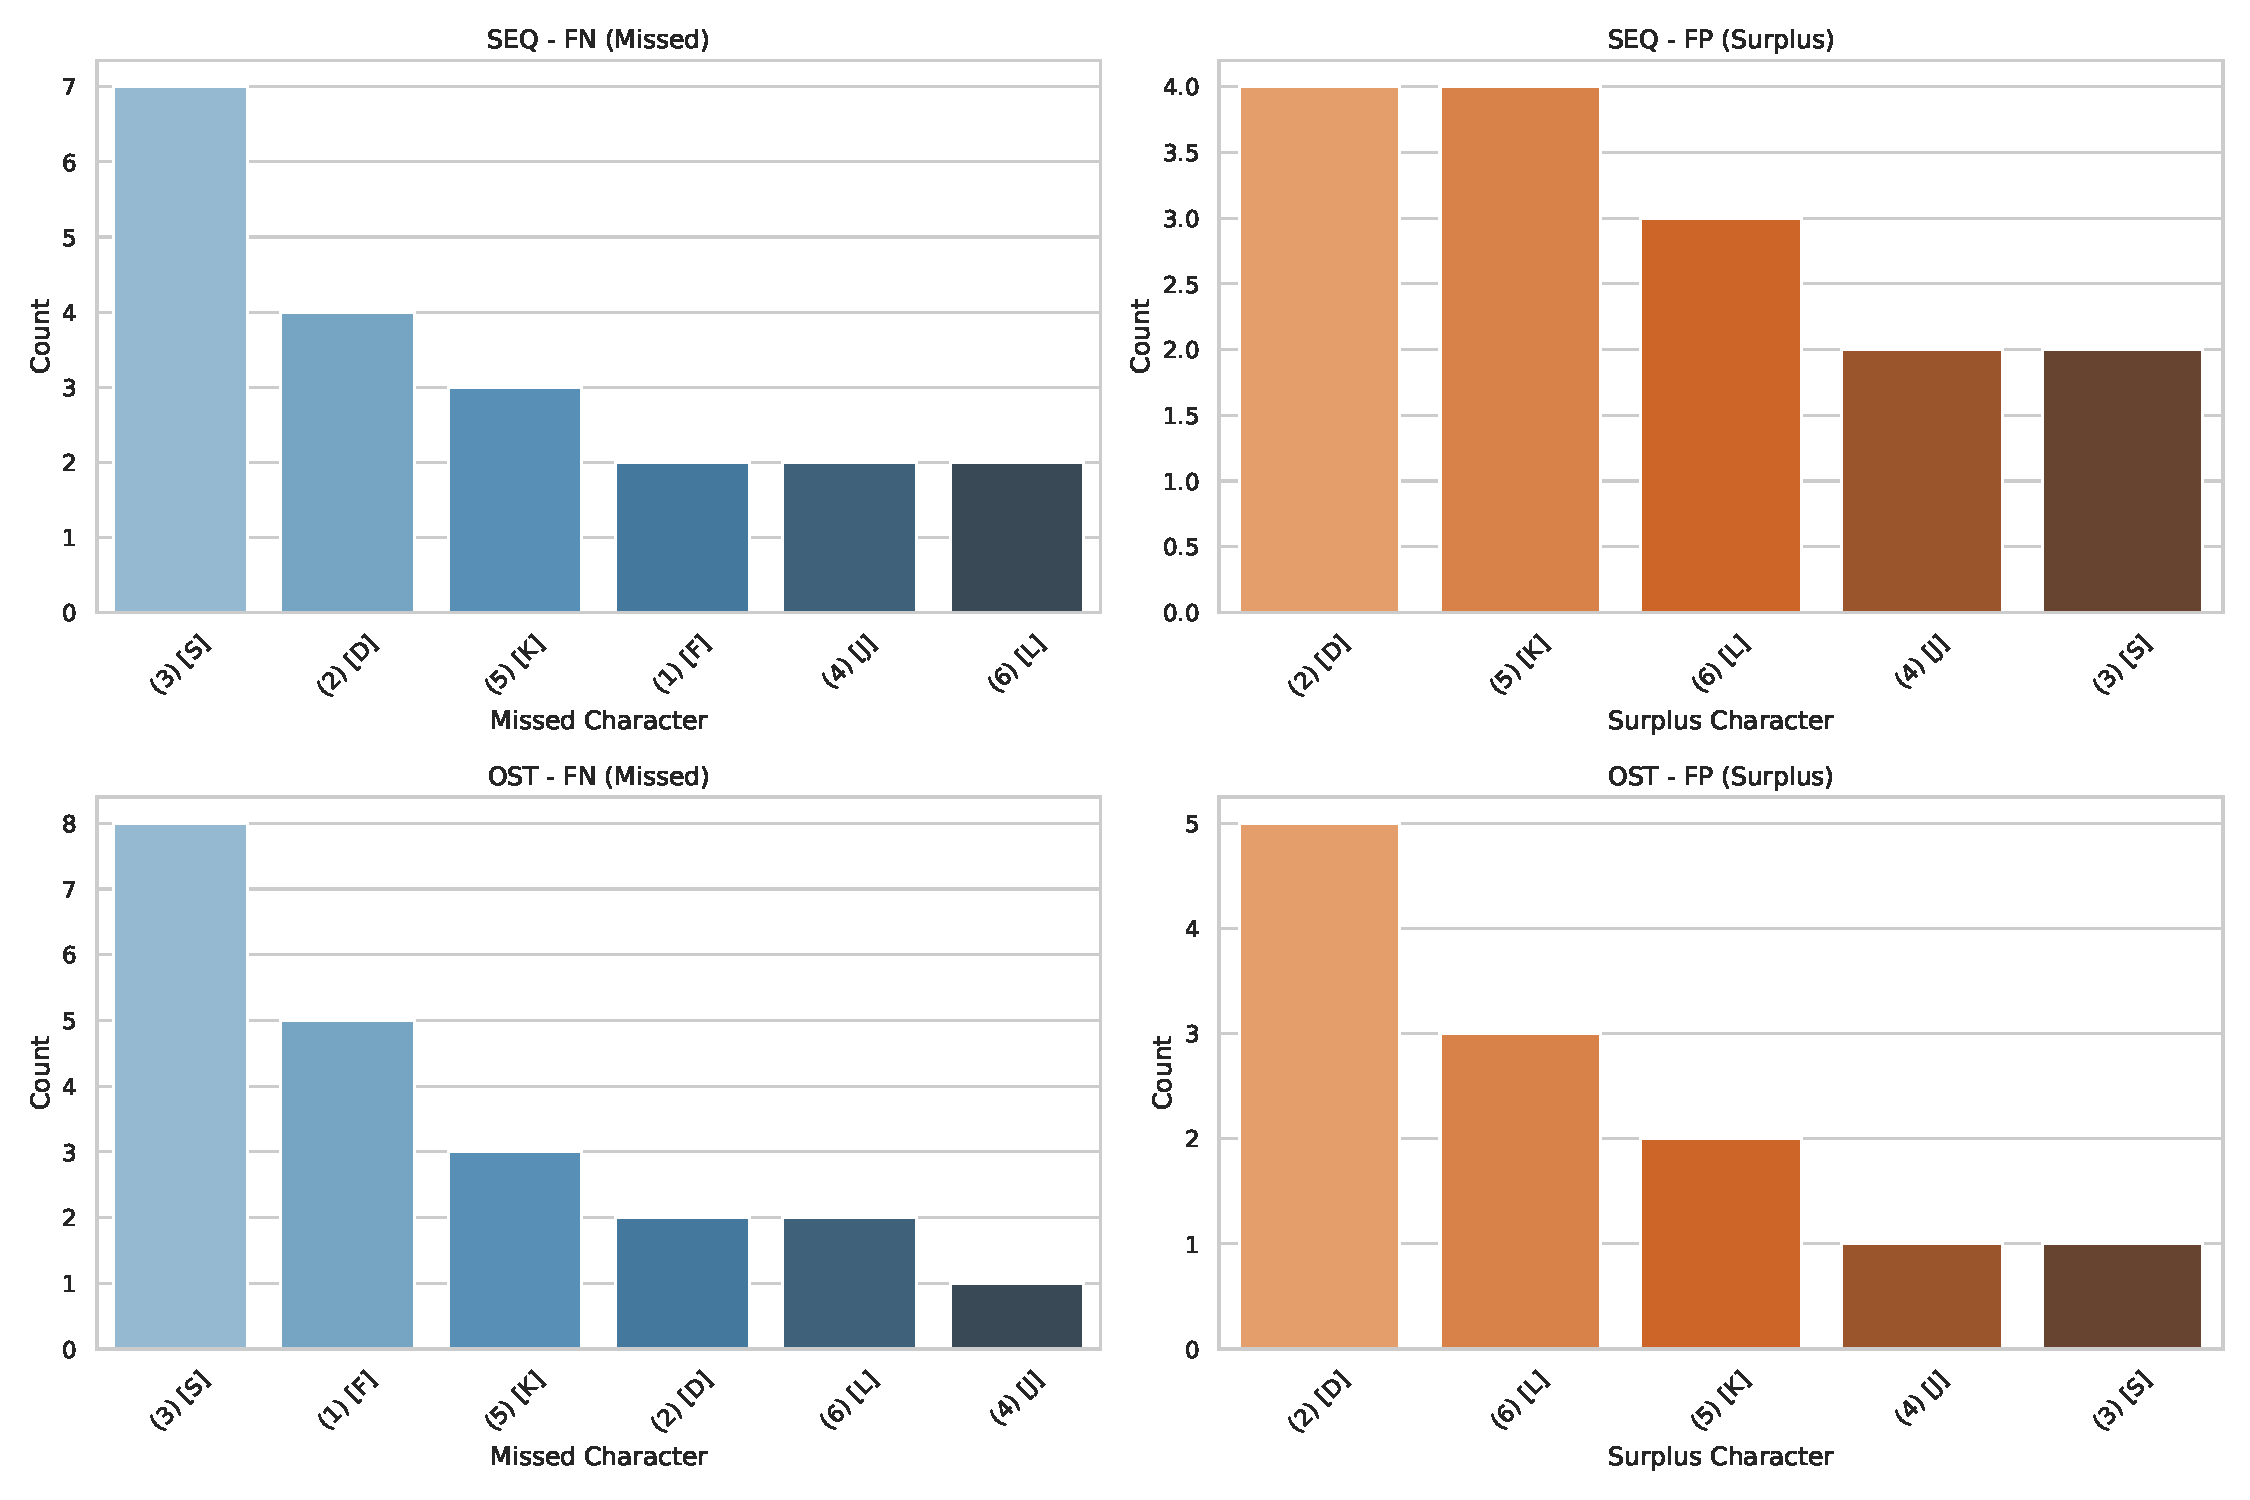
\includegraphics[width=\linewidth]{src/pictures/Study2Data/missed_surplus_test_study2.pdf}


S[3] often FN
J[4], L[6] least FN
D[2] often FP
S[3],J[4] least FP
means S = often pressed
J was almost everytime pressed when it needed to be

    \item (We analysed the errors given a Braille Character from the test-words)

        \centering
        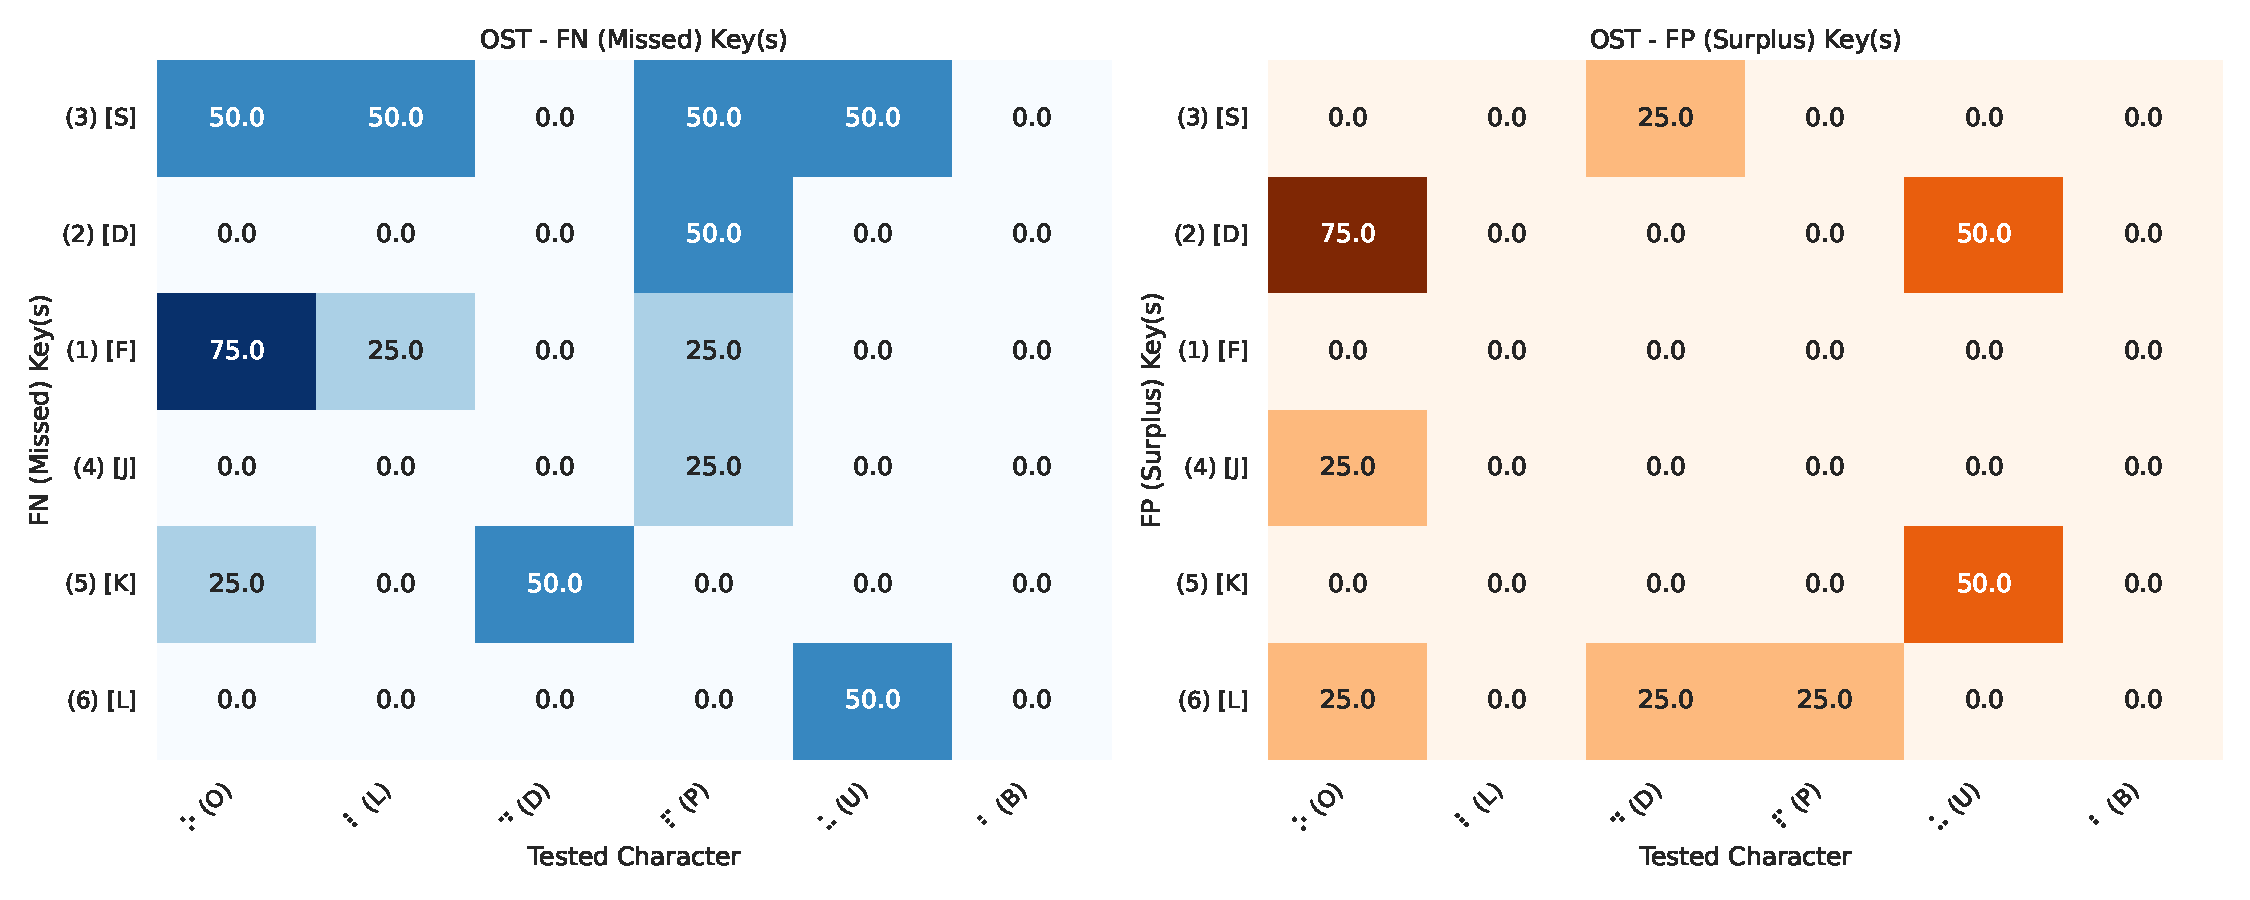
\includegraphics[width=\textwidth]{src/pictures/Study2Data/missed_surplus_test_percentages_study2_ost.pdf}
OST:

        \centering
        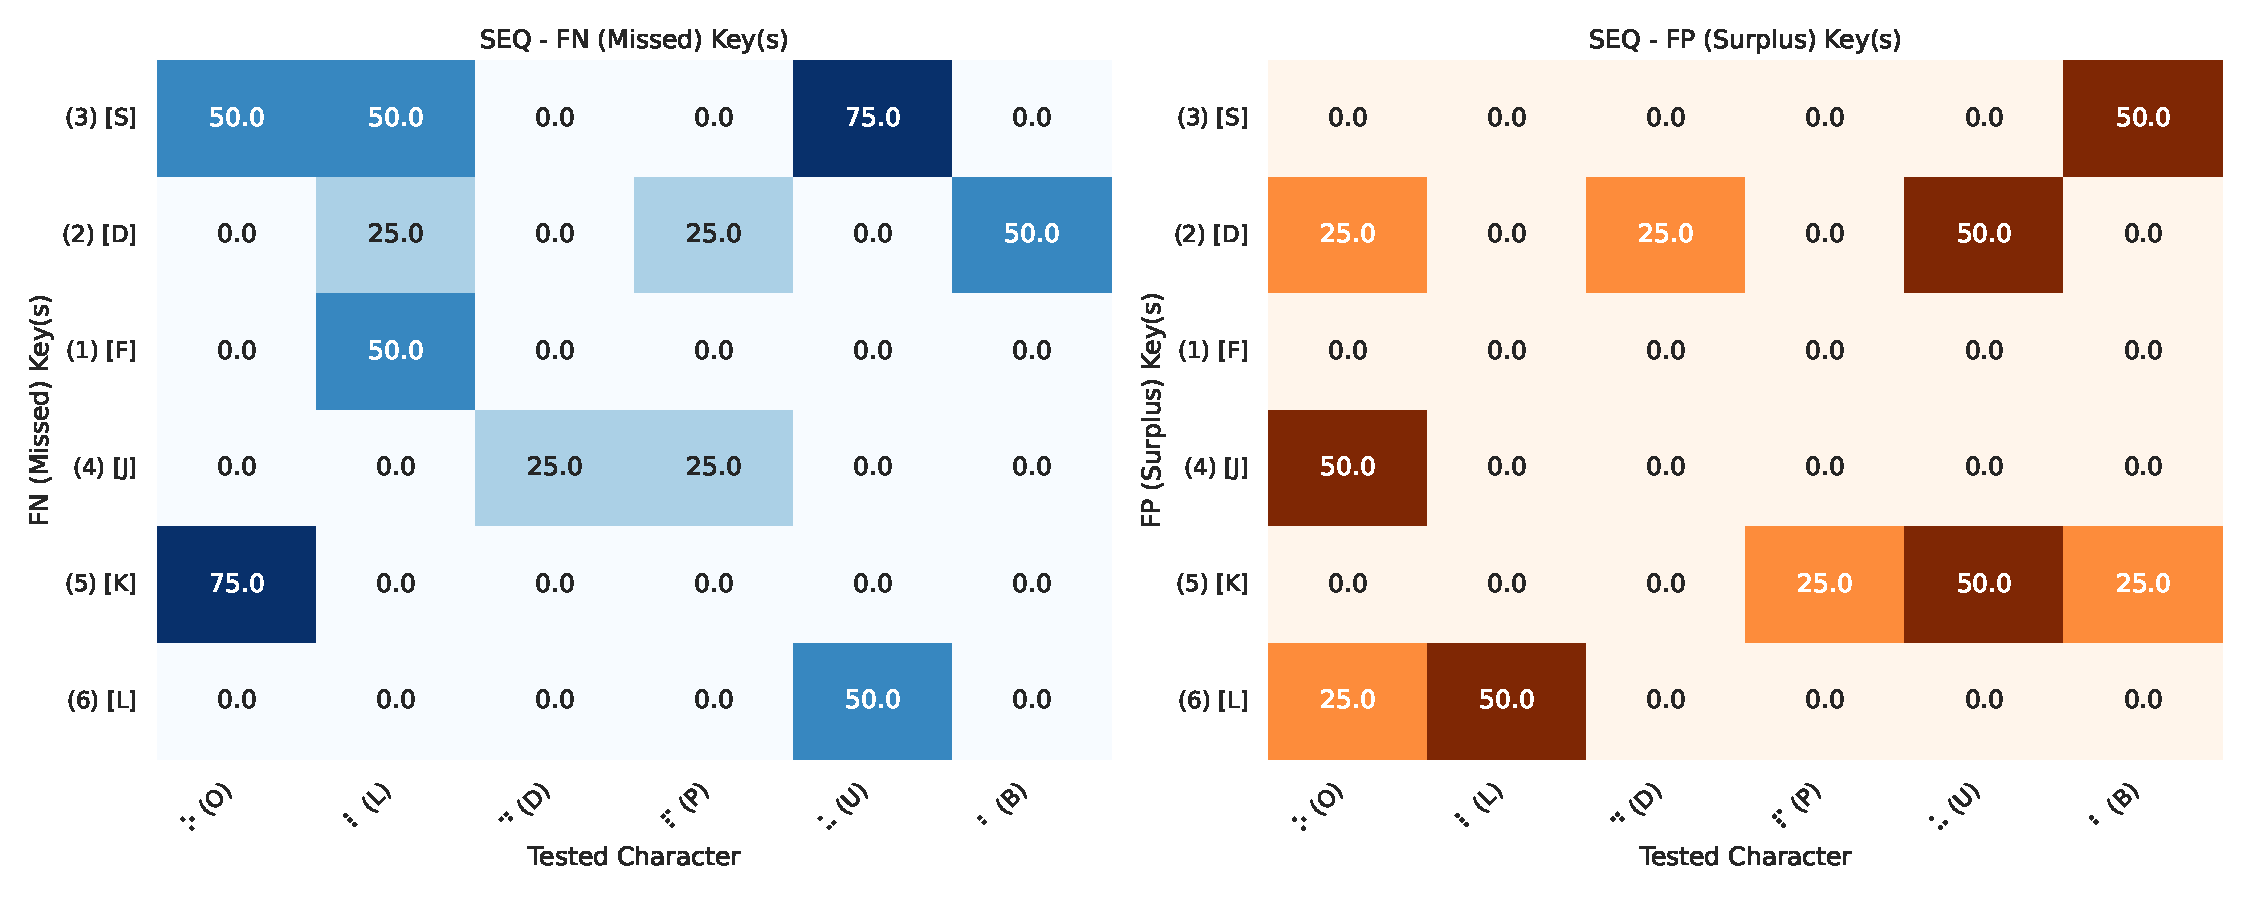
\includegraphics[width=\textwidth]{src/pictures/Study2Data/missed_surplus_test_percentages_study2_seq.pdf}
    SEQ:
    

    \item (In order to see the largest error-difference for the characters more visually appealing and using a cosine Similarity as it is comon in NLP word comparissons we plotted the PCA plots.)

    \centering
    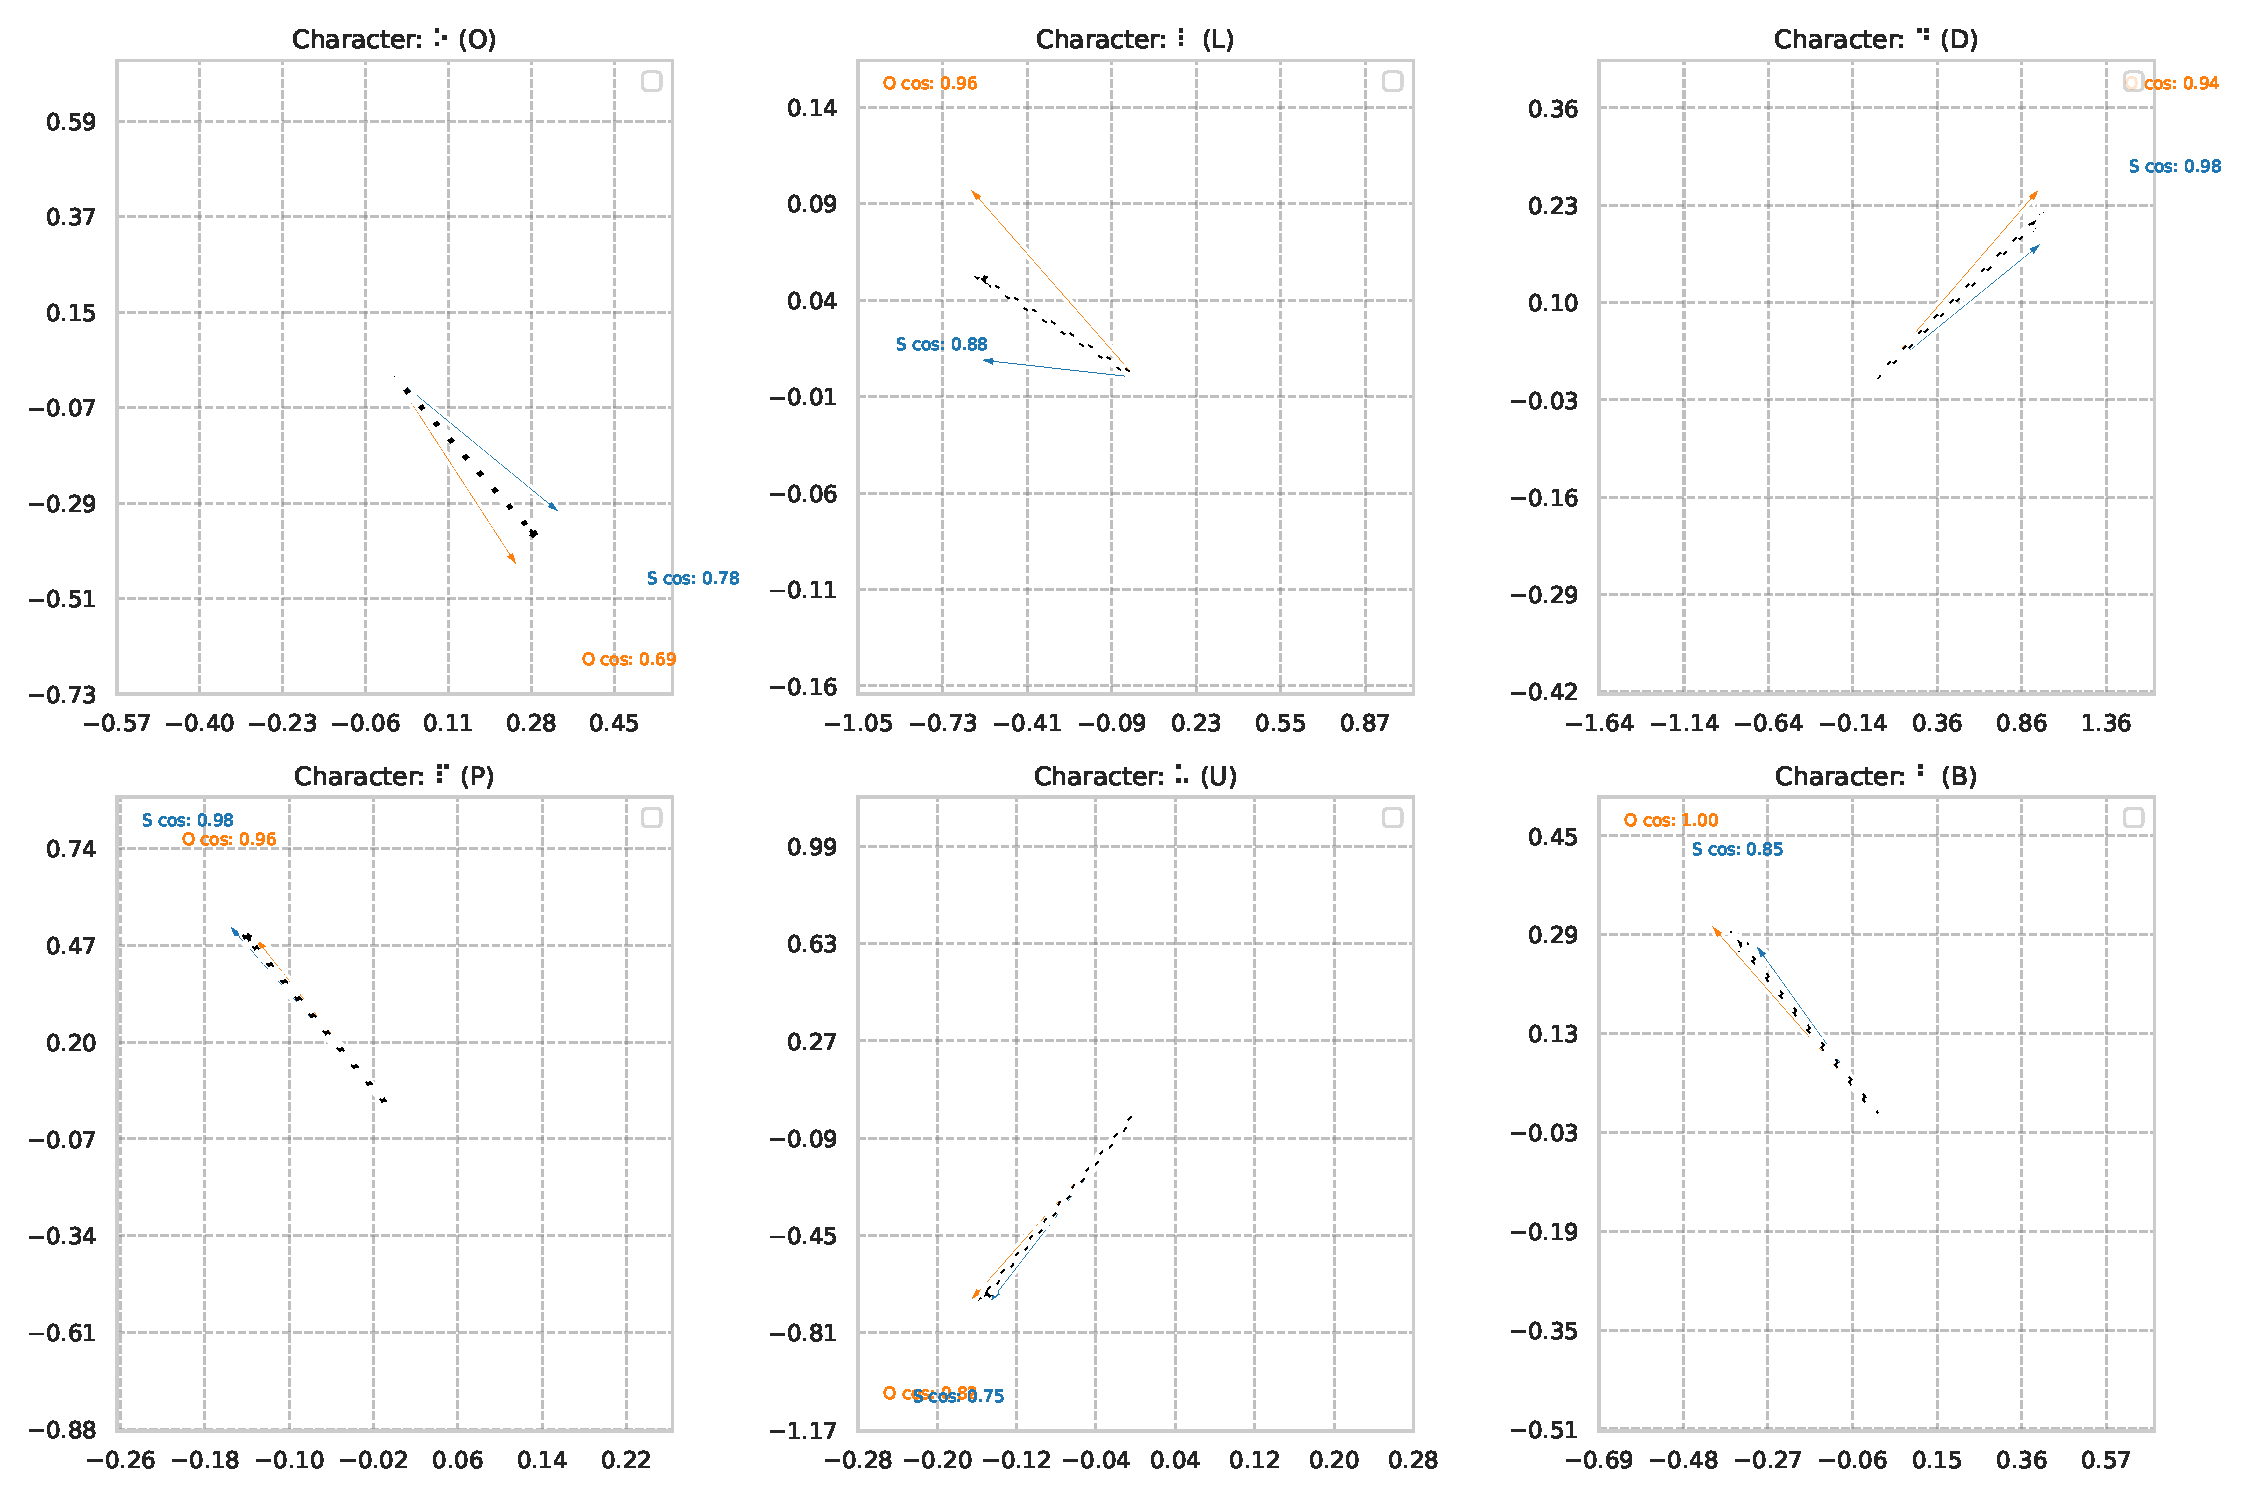
\includegraphics[width=\linewidth]{src/pictures/Study2Data/Vectors_study2.pdf}

    \item After passively Learning with a stimulus we conducted a NASA TLX for the task-load

    \centering
    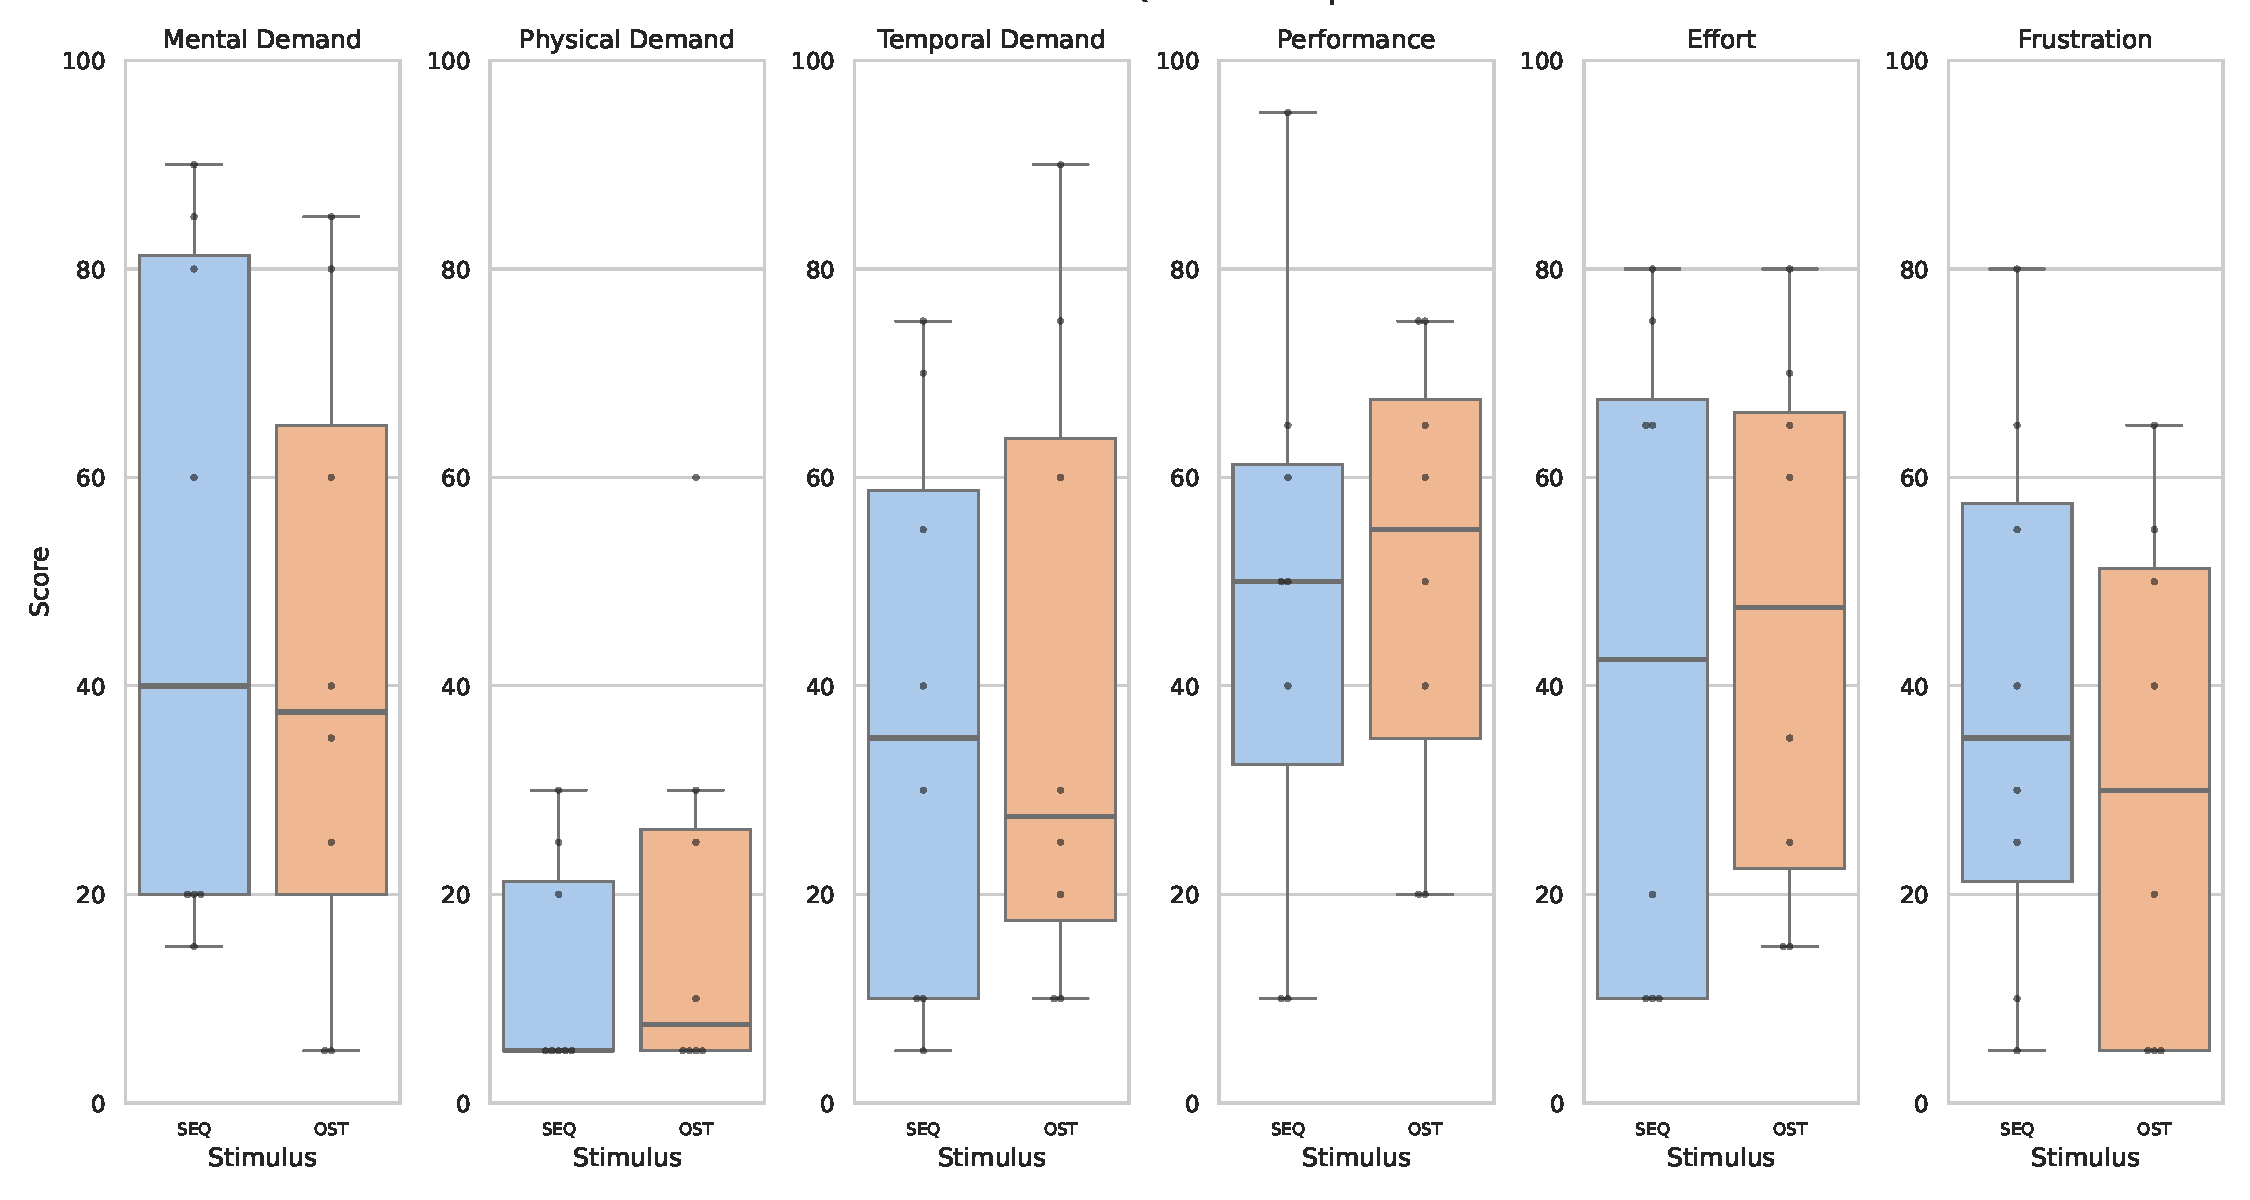
\includegraphics[width=\linewidth]{src/pictures/Study2Data/nasaTLX_study2.pdf}


\begin{table}[ht]
\resizebox{\columnwidth}{!}{
\centering
\begin{tabular}{|l|l|l|l|l|}
\hline
\textbf{Question} & \textbf{Test Statistic} & \textbf{p-value}  &\textbf{Significance}           &\textbf{Effect Size}\\ \hline
\textbf{Mental Demand}        & 35.500& 0.7513&Not Significant &0.2141\\ \hline
\textbf{Physical Demand}      & 27.000& 0.6019&Not Significant &0.3559\\ \hline
\textbf{Temporal Demand}      & 29.0000& 0.7911&Not Significant &0.1065\\ \hline
 \textbf{Performance}          & 27.5000& 0.6721&Not Significant &0.1228\\\hline
 \textbf{Effort}               &  27.500& 0.672&Not Significant &0.1285\\\hline
 \textbf{Frustration}          & 39.0000& 0.4907&Not Significant &0.3168\\\hline
\end{tabular}}
\caption{Results of \gls{mwu} significance tests for the different NasaTLX dimensions with Cohens d.}
\label{table:nasaTLX_significance_secondStudy_nonParam}
\end{table}

nasatlx similar for both encodings -> no difference in the task load

        \item Also we conducted asked the participants to rate the usefulness and satisfaction about the current Stimulus

    \centering
    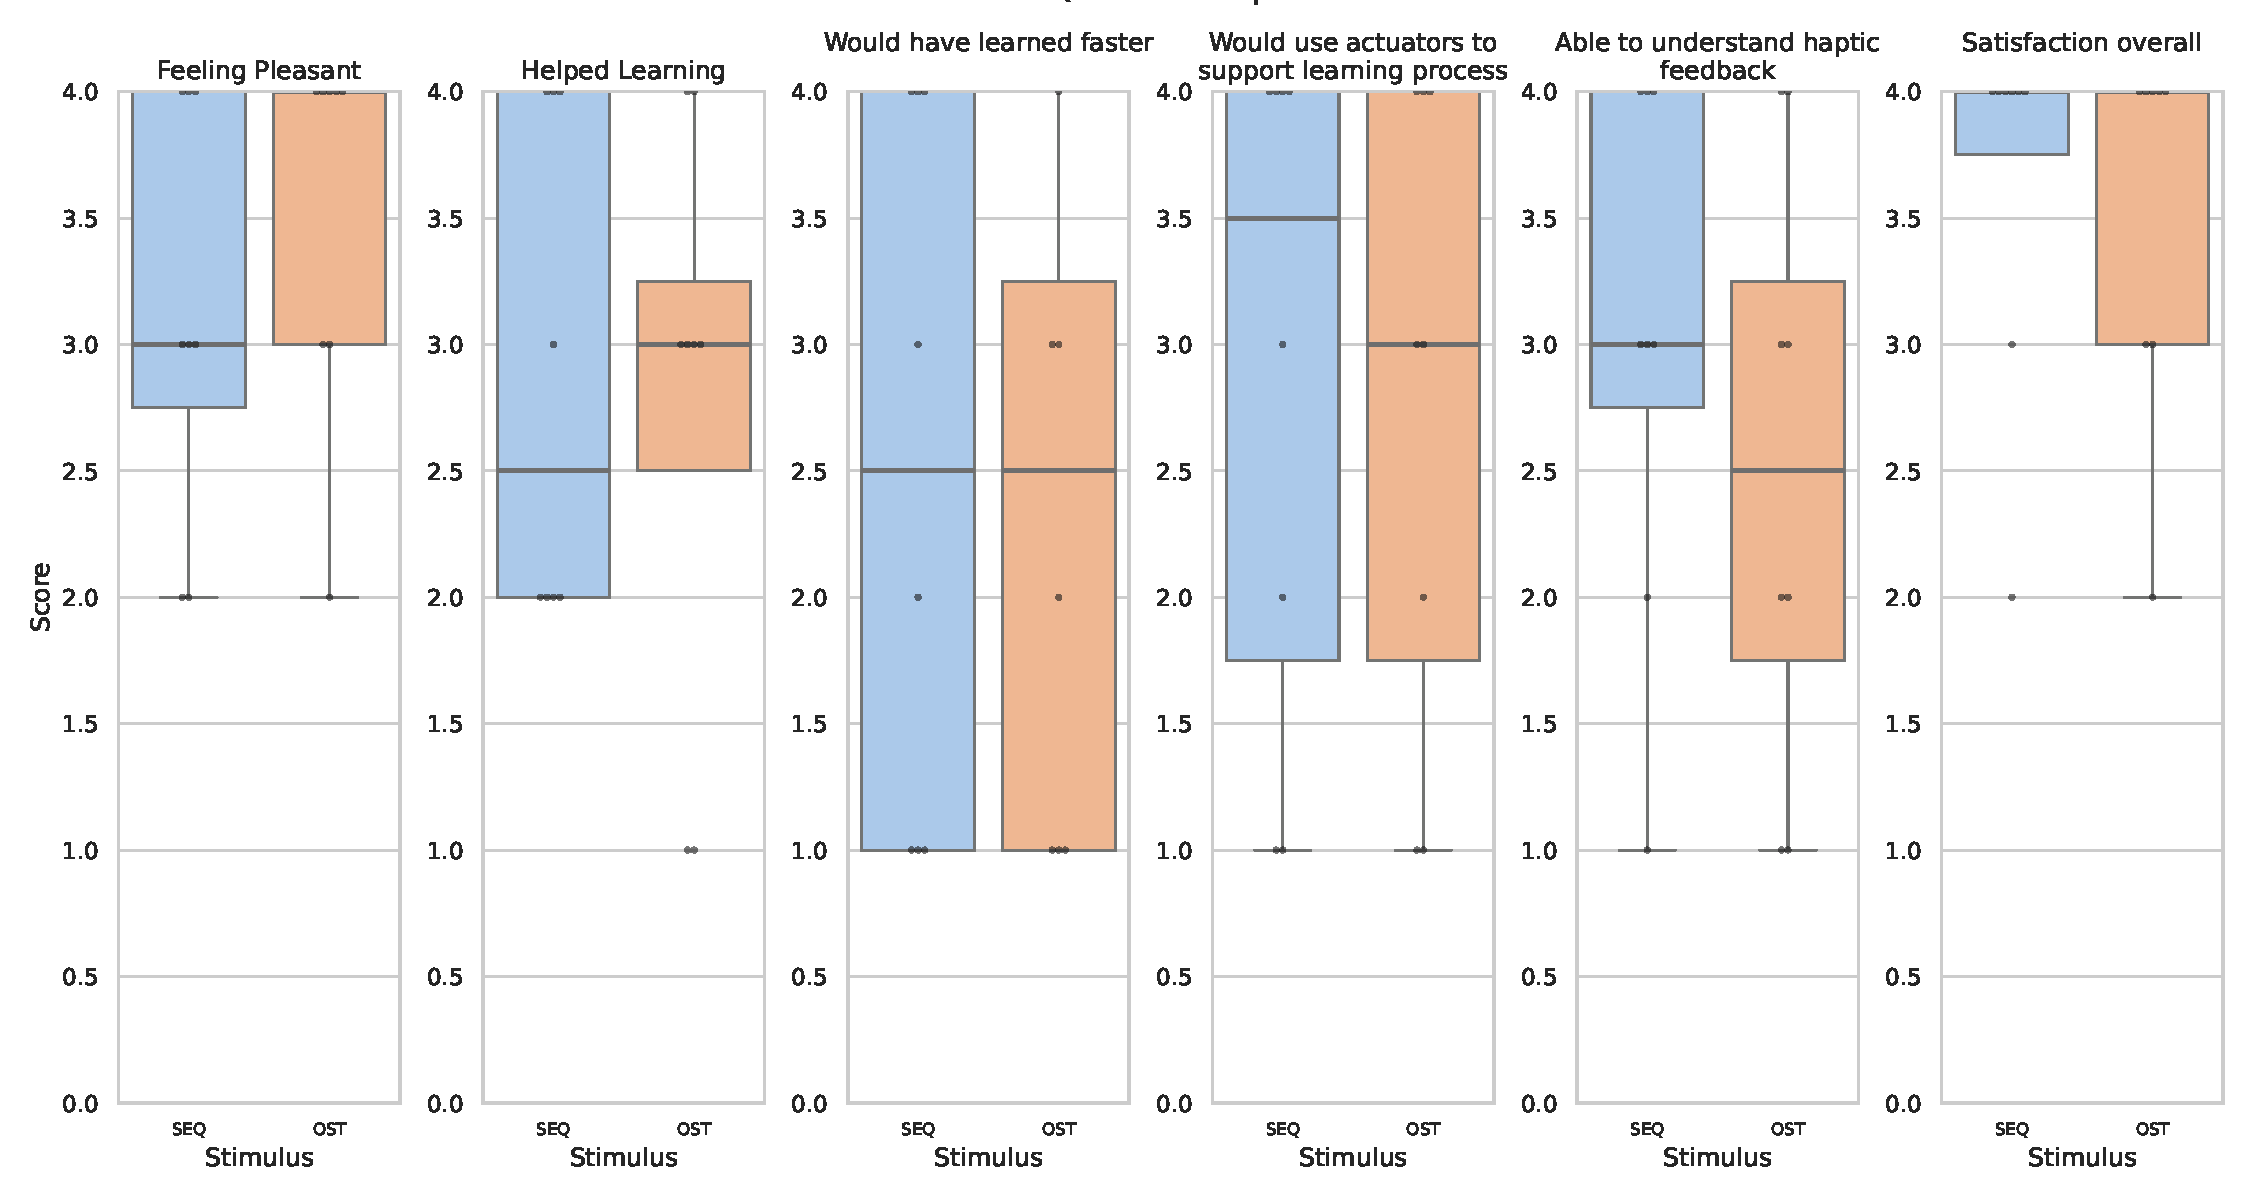
\includegraphics[width=\linewidth]{src/pictures/Study2Data/questions_special_study2.pdf}


\begin{table}[ht]
\resizebox{\columnwidth}{!}{
\centering
\begin{tabular}{|l|l|l|l|l|}
\hline
\textbf{Question} & \textbf{U-statistic}& \textbf{p-value}  &\textbf{Significance}           &\textbf{Effect Size}\\ \hline
\textbf{Feeling Pleasant}& 23.5000& 0.3596&Not Significant &0.2232\\ \hline
\textbf{Helped Learning}& 33.0000& 0.9565&Not Significant &0.0263\\ \hline
\textbf{Would have learned faster}& 32.5000& 1.000&Not Significant &0.0131\\ \hline
 \textbf{Would use actuators to support learning process}& 34.5000& 0.8244&Not Significant &0.0656\\\hline
 \textbf{Able to understand haptic feedback}&  40.0000& 0.4139&Not Significant &0.2100\\\hline
 \textbf{Satisfaction overall}& 35.5000& 0.7001&Not Significant &0.0919\\\hline
\end{tabular}}
\caption{Results of the \gls{mwu} test for significance grouped by the different self-assessment dimensions with a Cohens d Effect Size.}
\label{table:individualQuestions_significance_secondStudy_nonPara}
\end{table}

ost more pleasant,
ost helped learning
seq understandable feedback
seq satisfaction better

    \item After conducting \textbf{ALL Experiments}, the participants were asked to compare the Simuli against one another

    \centering
    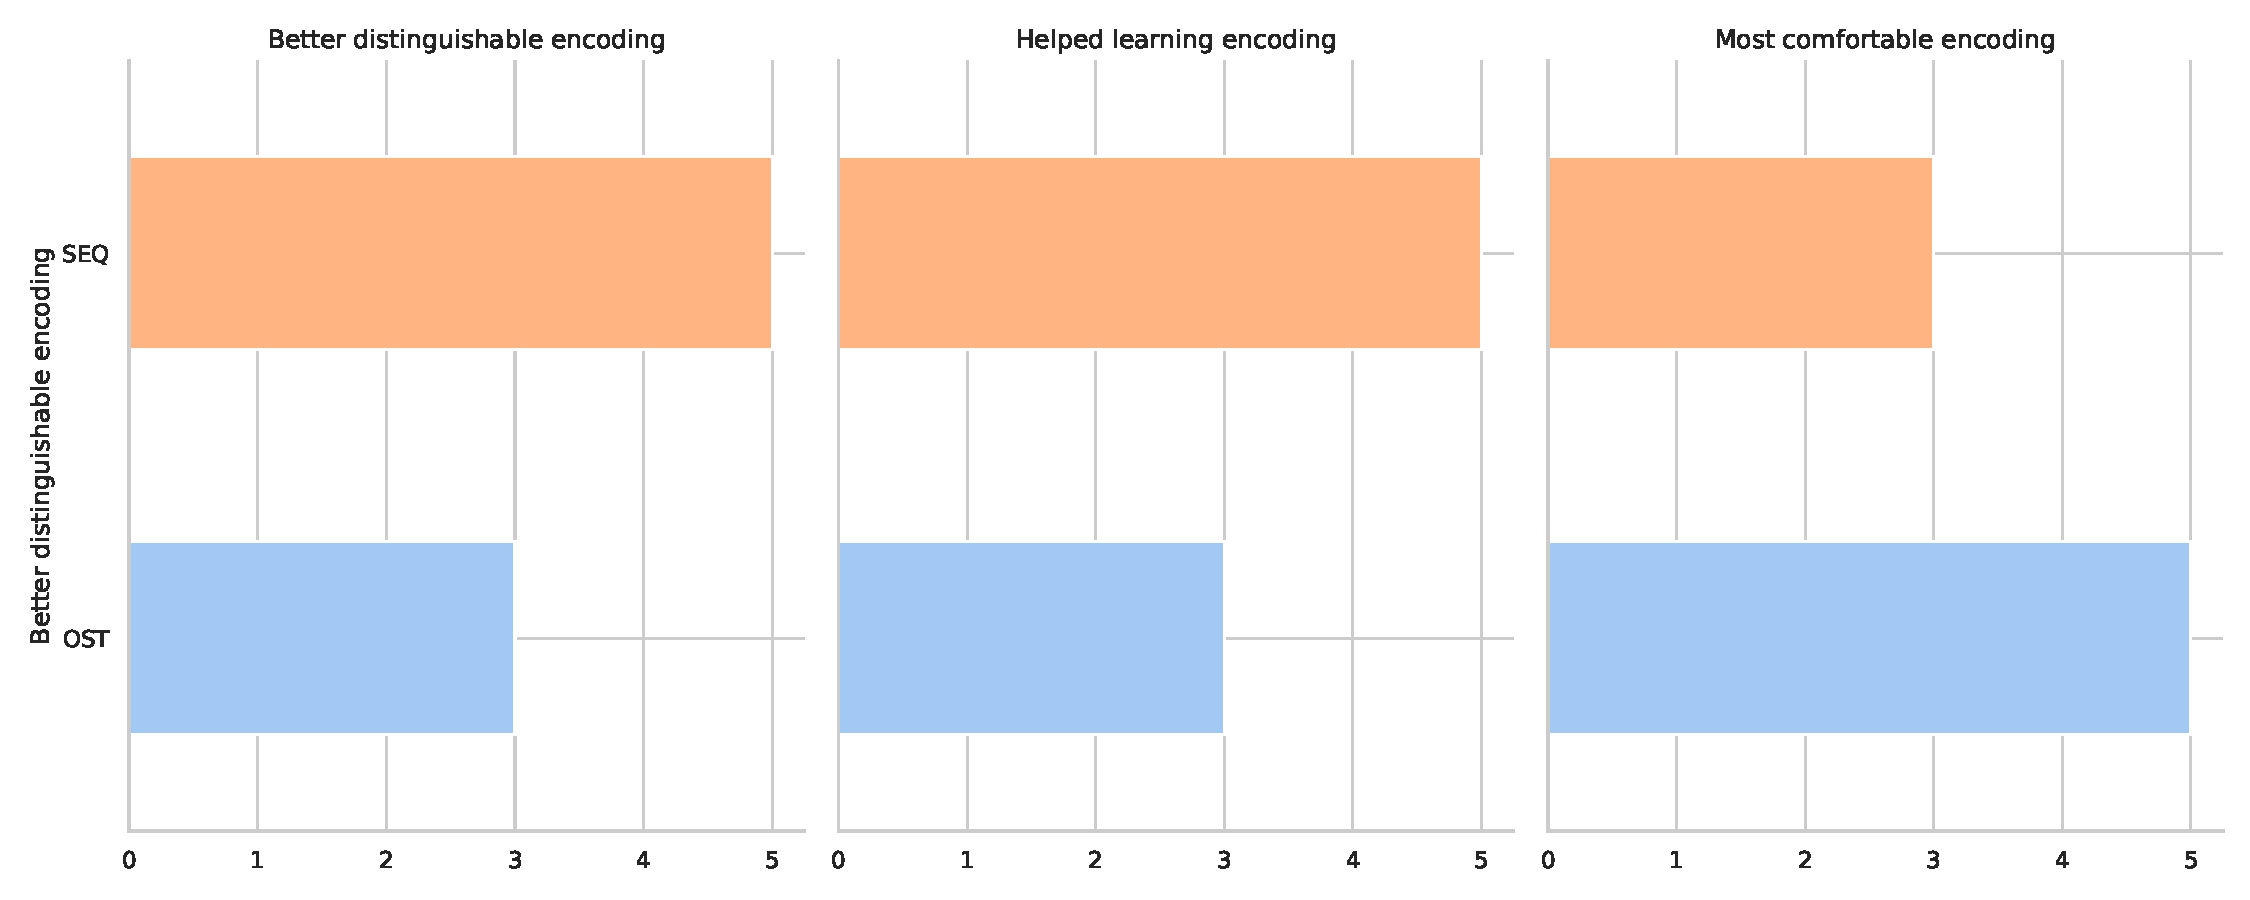
\includegraphics[width=\linewidth]{src/pictures/Study2Data/questions_compare_study2.pdf}

\begin{table}
\resizebox{\columnwidth}{!}{
    \centering
    \begin{tabular}{|c|c|c|c|}\hline
        Question & \gls{csgf} & p-value & Significance \\\hline
         \enquote{Better distinguishable encoding} & 0.5 & 0.4795& Not Significant\\\hline
         \enquote{Helped Learning encoding} & 0.5 & 0.4795 & Not Significant\\\hline
         \enquote{Most comfortable encoding}& 0.5 & 0.4795 & Not Significant\\\hline
    \end{tabular}}
    \caption{Statistical \gls{csgf} Results for the direct comparison between the stimuli.}
    \label{table:statistical_tests_comparrisson_secondStudy}
\end{table}
seq helped learning, distinguishable, but not comfortable

\item \textbf{Open Feedback}

\resizebox{\columnwidth}{!}{
\begin{tabular}{| l |}
\hline
Bei Ost erkenne ich die vibration nicht so akkurat \\
\hline
Für a-muster sehr gut \\
\hline
I had difficulties to register which finger did vibrate

it was somewhat distracting \\
\hline
Make it schön \\
\hline
ost was easier to ignore. Seq was harder to ignore, more irritating during the game.\\

anmerkung wrt. previous answers: bin grundsaetzlich der meinung, dass dinge aus buerchern zu lernen besser ist als fancy spiele.\\ daher die negative bewertung an der stelle,\\ ob wohl ich den spielerischen aspekt der uebung sehr cool fand. \\

das spiel war gegen ende ermuedend. 

wenn ich mit einer methode lernen muesste mit dem ziel am ende was gelernt zu haben,\\ wuerde ich SEQ waehlen.\\ wenns nur um  den spaß geht wuerde is OST waehlen. \\

fazit: hat spaß gemacht.\\

signale waren an der maus hand weit schlechter zu erkennen als an der hand, die nicht an der maus waren (also links)\\ meiner meinung nach weil die maus hand (rechts) in bewegungn war,\\ waehren die andere hand (links) still war und evtl, auch,\\ weill ich durch das halten der maus die finger naeher bei einander hatte, waehrend ich die finger der linken hand schoen spreizen konnte.  \\
\hline
In the second section I learned the braille better because the devices of each finger didn’t vibrate at the same time \\
\hline

\end{tabular}}

\end{enumerate}

ost vibration is bad
seq is better for learning but distracts

\textbf{Results}
SEQ is mostly better due to the distinguishability, but not by a long shot.
Ost is more comfortable.
Ost was better for one hand, but seq for two hands